\chapter{An Immersed-Boundary Approach for Multilayer Ice Accretion Simulations}\label{sec:ibmArticle}

\textit{
    This chapter presents an immersed-boundary framework for aircraft ice accretion simulations. The methodology uses a signed-distance level-set representation of the geometry, with the immersed-boundary formulation applied to both the RANS flow solver and the Eulerian and Lagrangian droplet impingement solvers on a non-conformal background mesh. A hybrid strategy is then adopted for ice-shape evolution, where the level-set-based geometry update is performed on adapted body-fitted meshes. The approach is assessed using a cylinder verification case, an impingement benchmark, and rime and glaze ice accretion cases on a NACA~0012 airfoil, and a 3D multilayer ice-accretion benchmark. The cylinder case confirms that the immersed-boundary droplet formulations recover the analytical collection-efficiency solution. The impingement benchmark shows good agreement with experimental collection-efficiency data, while the rime and glaze cases demonstrate that the ice shapes agree well with experimental measurements. The final case demonstrates the complete immersed-boundary multilayer methodology on a 3D benchmark configuration.
}

\section{Introduction}
\label{ibm:sec:introduction}

The numerical ice-accretion workflow and its principal physical components, namely the aerodynamic flow, droplet impingement, surface thermodynamics, and geometry evolution, have been introduced in the literature review (Section~\ref{sec:review_icing_overview}). In a conventional body-fitted framework, successive accretion layers require the computational mesh to conform to the evolving ice surface. This requirement can become increasingly restrictive as complex ice geometries develop. \removeText{To address these constraints, this chapter focuses on the implementation and assessment of an immersed-boundary icing framework within \textsc{CHAMPS}. The solid surface is embedded in a non-conformal background mesh. The immersed-boundary flow solver was developed prior to this work and is presented here for completeness, while both Eulerian and Lagrangian droplet solvers are adapted to the immersed geometry. The thermodynamic model remains surface based, and geometry evolution is performed with the continuous level-set methodology presented in Chapter~\ref{sec:lsArticle}.}

\addText{Immersed-boundary methods have been investigated as an alternative to repeated body-fitted remeshing in ice-accretion simulations. Among the pioneering developments, Capizzano et al.~\cite{capizzano2014eulerian,capizzanoIcing} developed a 3D multistep ice-accretion framework employing discrete-forcing immersed-boundary methods for both the RANS aerodynamic and Eulerian droplet equations, with ice-shape evolution performed through Lagrangian displacement of surface nodes. Lavoie et al.~\cite{lavoieDroplets, lavoie2021immersed} investigated a penalization approach for both the inviscid aerodynamic flow and Eulerian droplet equations, restricting their developments to 2D geometries. While the droplet formulation provided accurate impingement predictions, the penalized flow treatment exhibited more restrictive convergence properties, with first-order spatial accuracy. Their icing methodology also incorporated an integral boundary-layer approach for heat-transfer estimation and a level-set method for ice-shape evolution. Building on these developments, Elices Paz et al.~\cite{pabloIcing, pabloThesis} extended the methodology to 3D multilayer ice accretion, retaining the penalized Eulerian droplet formulation while adopting a ghost-cell treatment for the aerodynamic equations. The ghost-cell methodology incorporated geometry-dependent positioning of ghost and image points to improve the reconstruction of flow variables near immersed boundaries. Ice-shape evolution was performed through Lagrangian displacement of surface nodes, with displacement directions obtained from the signed-distance field normals. Al-Kebsi et al.~\cite{alkebsiPhd} investigated a level-set-based approach to multistep ice accretion, combining an implicit representation of the evolving ice surface with a penalization-based RANS solver for the aerodynamic flow and a ghost-cell approach for Eulerian droplet impingement. Particular attention was devoted to the associated difficulties of interface preservation and mass conservation during level-set advection in an immersed-boundary framework.}

\addText{In this work, the immersed-boundary capabilities of \textsc{CHAMPS} are extended to accommodate the complete ice-accretion process. An existing ghost-cell RANS solver, developed independently of this work, is employed for the aerodynamic calculations and presented here for completeness. For droplet impingement, the penalization strategy previously demonstrated by Lavoie et al.~\cite{lavoieDroplets} is adopted for the Eulerian formulation, while the Lagrangian solver developed in Chapter~\ref{sec:lagArticle} is extended to detect impacts directly on the immersed surface. The thermodynamic model remains surface based and therefore requires no further modification to accommodate the immersed-boundary representation. Geometry evolution is performed using the continuous level-set methodology presented in Chapter~\ref{sec:lsArticle}.}

The resulting strategy is hybrid: the flow and droplet solutions are performed on the background IBM mesh, whereas the geometry-evolution problem is solved on its own adapted body-fitted mesh. This arrangement removes the need to repeatedly generate or deform a body-fitted RANS mesh during multilayer accretion, thereby alleviating the more restrictive mesh-generation requirements associated with the flow and droplet solvers. Such constraints are considerably less limiting for the level-set problem, for which suitable adapted meshes can be generated more readily. \addText{Furthermore, retaining a body-fitted representation for the level-set calculation allows geometry evolution to be restricted to the ice-accretion region, avoiding unintended displacement of ice-free portions of the immersed surface.}

The chapter first describes the immersed-boundary representation, flow treatment, and droplet formulations in Sections~\ref{ibm:sec:ibmRepresentation}--\ref{ibm:sec:dropSolver}, followed by their coupling with the thermodynamic and geometry-evolution models in Section~\ref{ibm:sec:thermoGeo}. The complete framework is then assessed in Section~\ref{ibm:sec:results} using a canonical cylinder impingement case, an SLD impingement benchmark, and rime and glaze ice-accretion cases on airfoils. Comparisons with body-fitted predictions and experimental data are used to isolate the effect of the immersed-boundary treatment. Finally, a 3D multilayer ice-accretion case is considered to demonstrate the complete immersed-boundary framework on a more complex configuration. The main findings are summarized in Section~\ref{ibm:sec:conclusions}.

\section{Immersed-Boundary Representation}
\label{ibm:sec:ibmRepresentation}

In the present chapter, the solid geometry is represented implicitly in the volume mesh using a signed-distance level-set function $\phi$:
\begin{equation}
\phi =
\begin{cases}
< 0, & \text{inside the solid region}, \\
= 0, & \text{at the immersed interface}, \\
> 0, & \text{inside the fluid domain}.
\end{cases}
\label{ibm:eq:levelSet}
\end{equation}
An example of the resulting signed-distance field around a circular cylinder is shown in Figure~\ref{ibm:fig:cylinderDistance}.

\begin{figure}[ht]
    \centering
    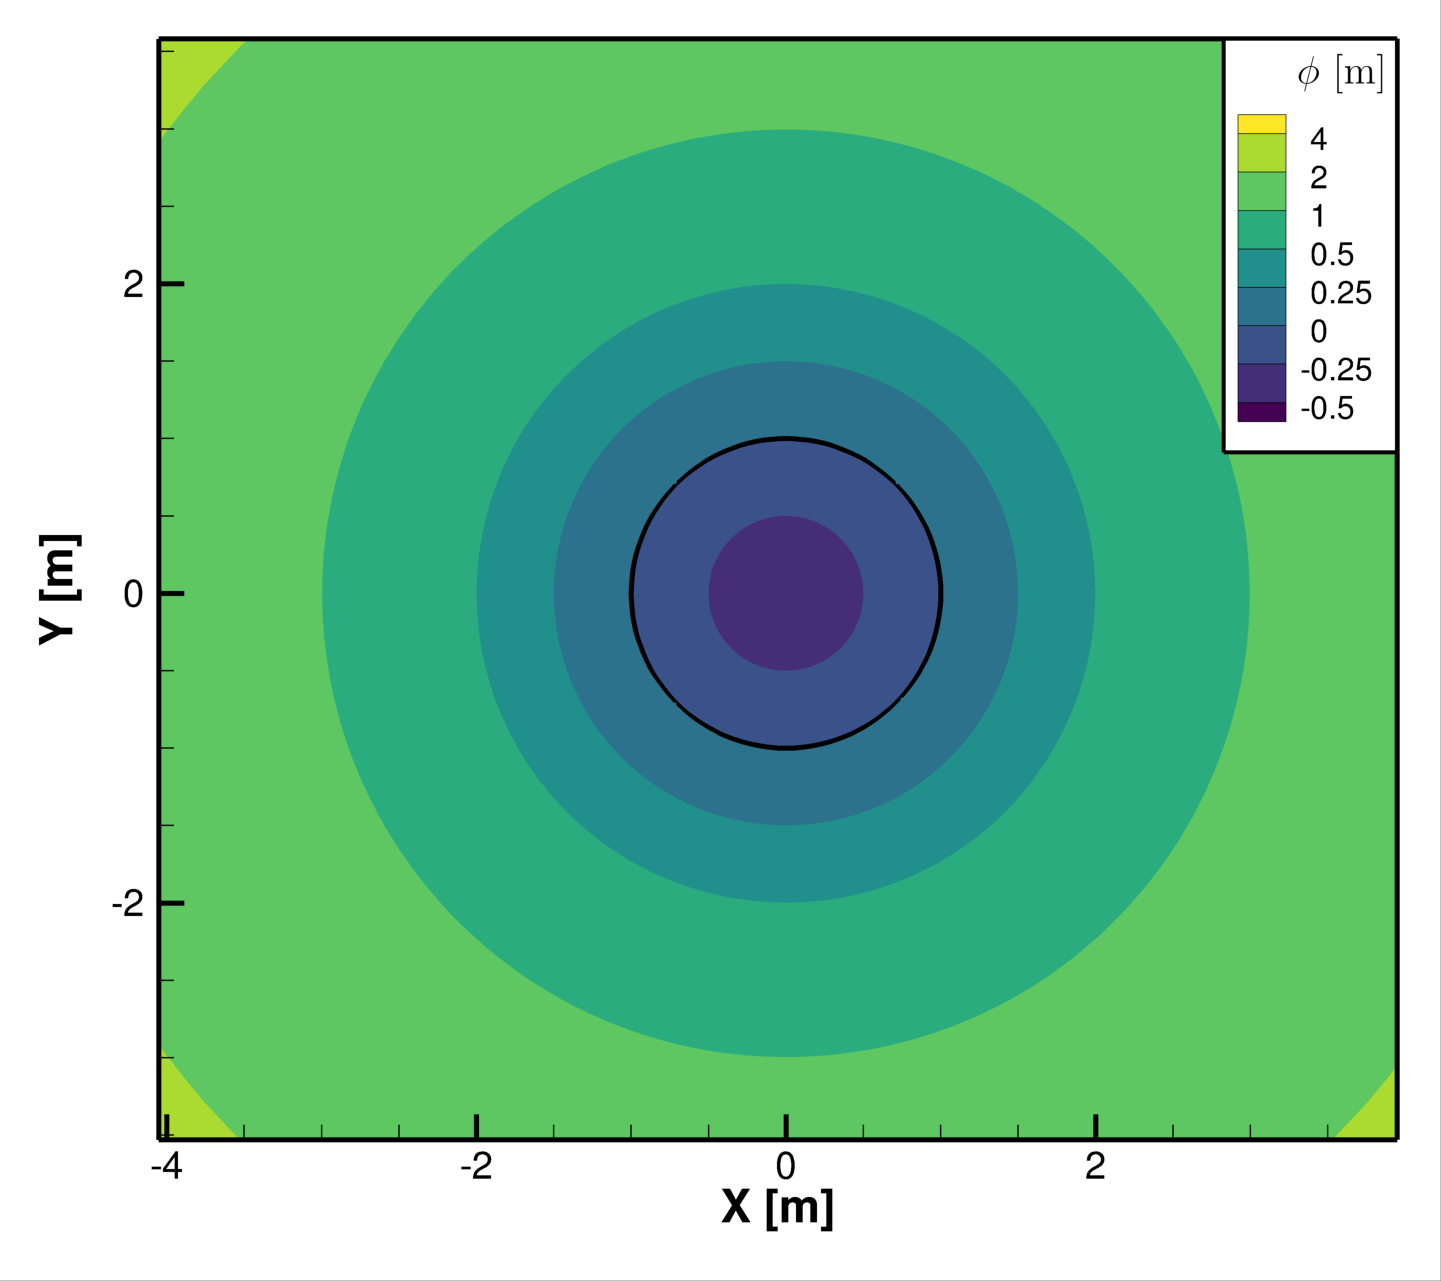
\includegraphics[trim={.1cm .1cm .1cm .1cm},clip,width=0.6\textwidth]{FIGURES/IBM_ARTICLE/CASE_CYLINDER_DISTANCE.png}
    \caption{Signed level-set field $\phi$ around a circular cylinder. The zero level set defines the cylinder surface, while positive values correspond to the fluid region and negative values to the solid region.}
    \label{ibm:fig:cylinderDistance}
\end{figure}

The initial level-set field is computed from the shortest distance between each volume-cell center and the immersed geometry. The sign of $\phi$ is determined using a ray-casting procedure \cite{schneider2002geometric}. The gradient of the level-set field is reconstructed using a weighted least-squares approach, from which the unit normal to the immersed interface is obtained as
\begin{equation}
    \boldsymbol{n}_{\phi} = \frac{\nabla \phi}{\left\| \nabla \phi \right\|}
    \label{ibm:eq:levelSetNormal}
\end{equation}
The resulting geometric information is used throughout the immersed-boundary framework, both to identify and classify cells relative to the immersed interface and to impose boundary conditions in the flow and Eulerian droplet solvers.

The geometric operations required by the immersed-boundary formulation involve repeated distance, closest-point, and intersection queries against the surface mesh. To accelerate these operations, an axis-aligned bounding-box (AABB) tree is constructed from the immersed-surface elements~\cite{schneider2002geometric}. Rather than subdividing the spatial domain, the AABB tree recursively partitions the surface elements into smaller groups and encloses each group within a tightly fitted bounding box. During a geometric query, complete branches of the tree can be discarded whenever their bounding boxes cannot contain a closer point or intersect the search segment, thereby avoiding explicit tests against the corresponding surface elements. This differs from a quadtree, which recursively subdivides the physical domain into four spatial regions independently of the distribution of the surface elements. As illustrated in Figure~\ref{ibm:fig:searchStructures} for a circular immersed surface, the AABB hierarchy remains concentrated around the surface geometry, whereas the quadtree partitions the surrounding domain, including regions containing no surface elements. \addText{For this example, 1,000 nearest-point queries were performed against a surface discretized using 256 segments. While a direct search requires 256 geometric tests per query, the AABB tree reduced this number to approximately 25, compared with 60 for the quadtree. Both hierarchical approaches therefore substantially reduce the search effort, with the AABB tree requiring fewer geometric tests in this configuration. This reduction is particularly relevant for 3D simulations involving larger surface meshes and repeated geometric queries, motivating the selection of the AABB tree for the present work.}
\begin{figure}[htbp]
    \centering
    \subfloat[AABB-tree decomposition.]{%
        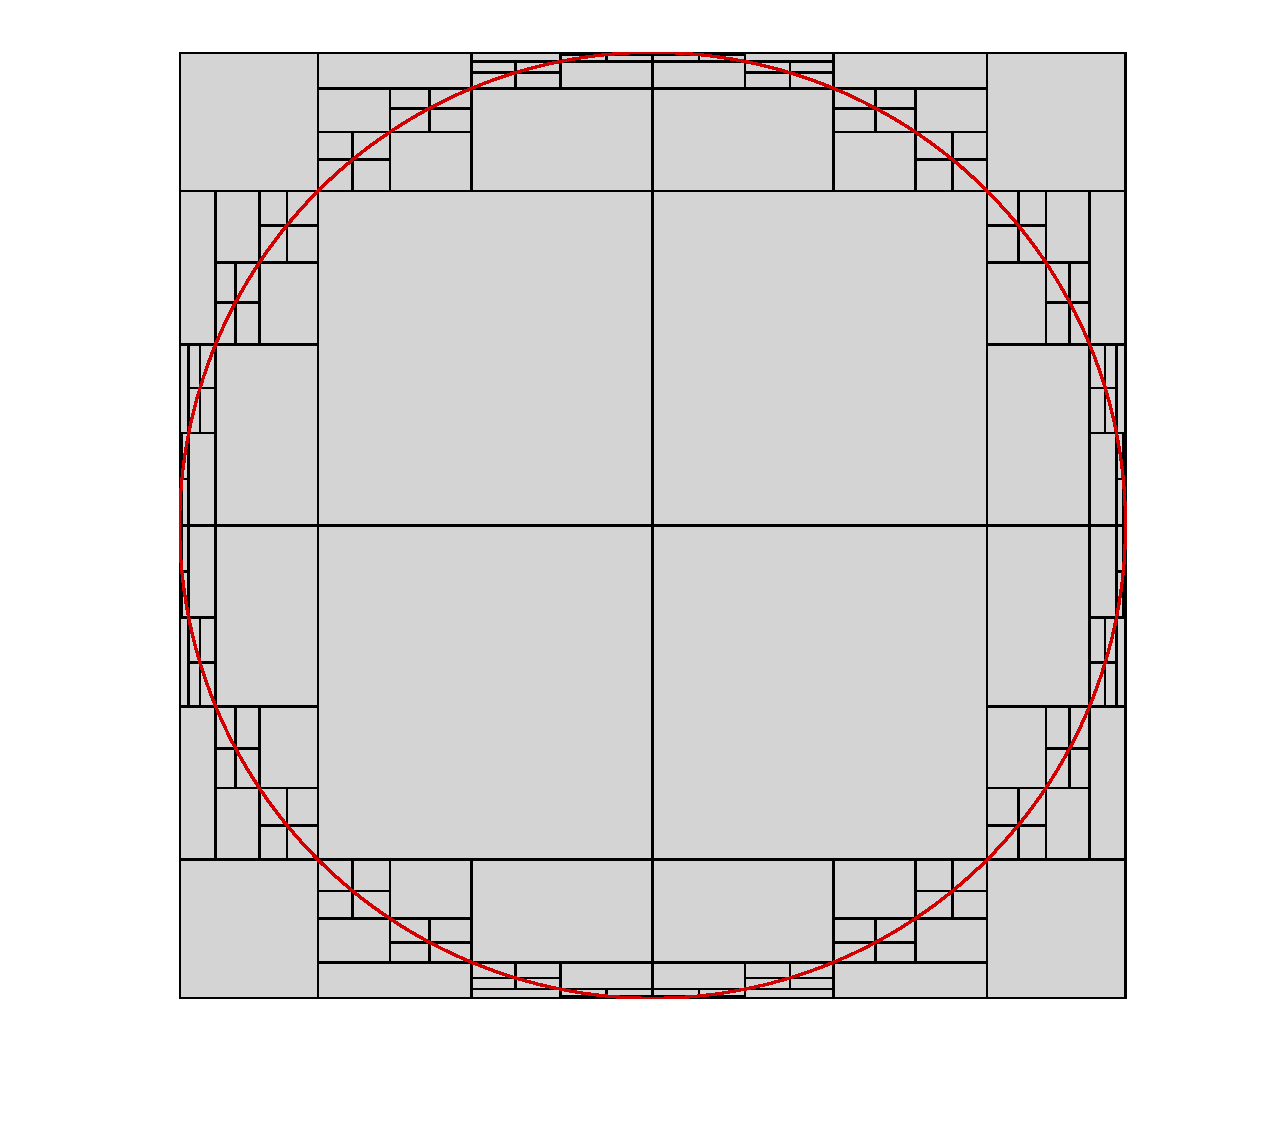
\includegraphics[width=0.48\textwidth]{FIGURES/IBM_ARTICLE/AABB_TREE.eps}
        \label{ibm:fig:aabbTree}%
    }
    \hfill
    \subfloat[Quadtree decomposition.]{%
        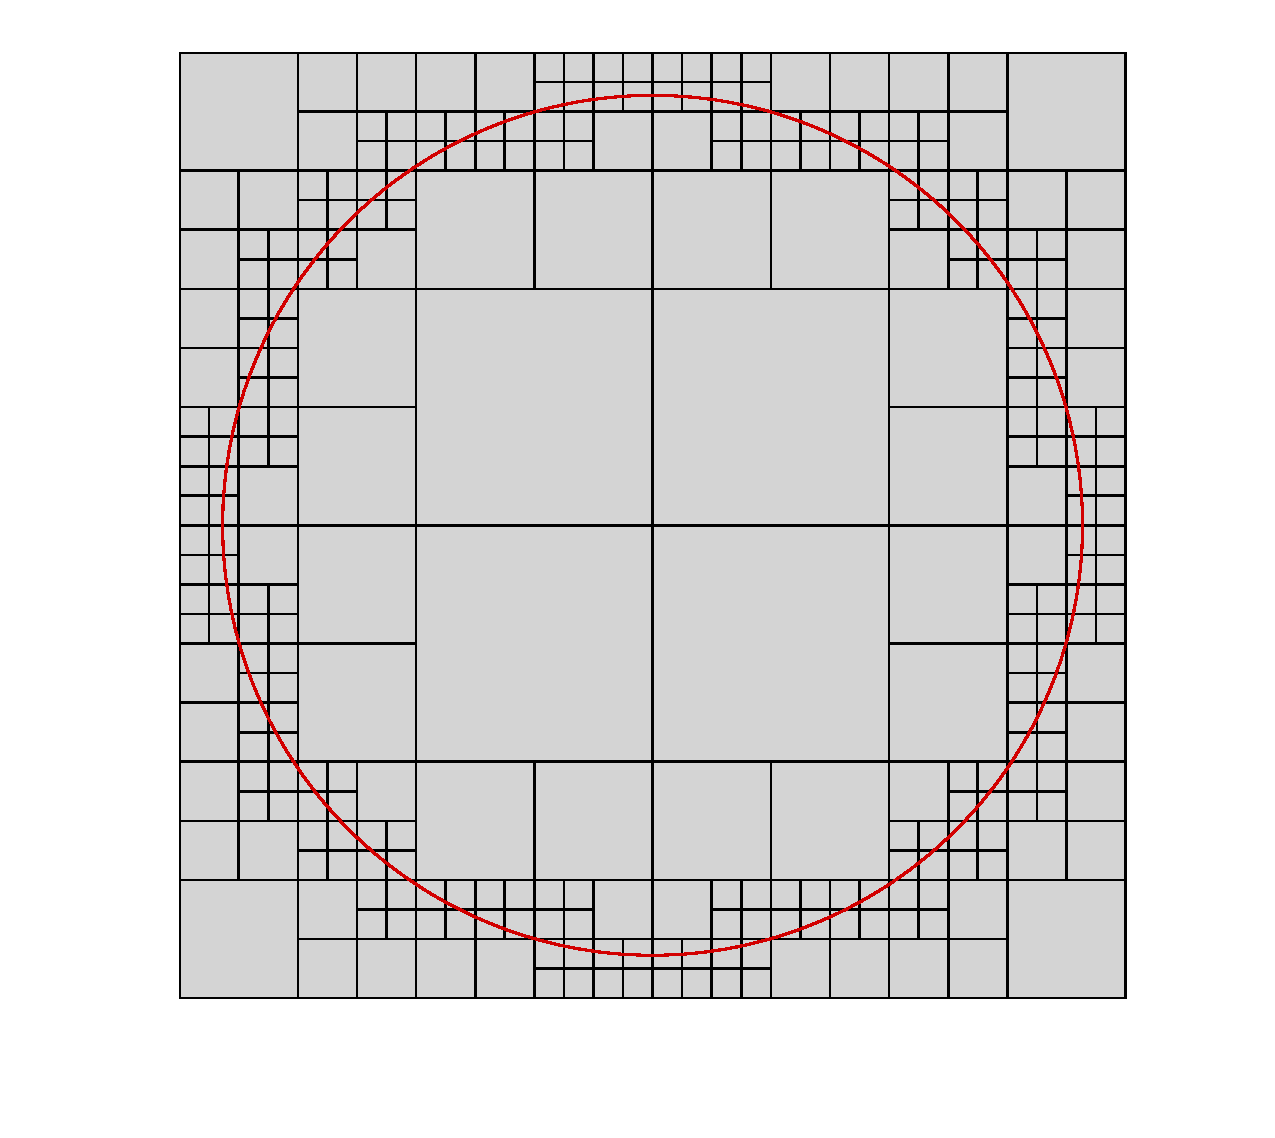
\includegraphics[width=0.48\textwidth]{FIGURES/IBM_ARTICLE/QUAD_TREE.eps}
        \label{ibm:fig:quadtree}%
    }
    \caption{Comparison of AABB-tree and quadtree search structures for a circular immersed surface. The AABB tree recursively partitions the surface elements and encloses each group within a bounding box, whereas the quadtree recursively partitions the surrounding spatial domain.}
    \label{ibm:fig:searchStructures}
\end{figure}
\removeText{As an illustrative example, 1,000 nearest-point queries were performed against the circular surface of Figure~\ref{ibm:fig:searchStructures}, discretized using 256 segments. A direct search requires 256 geometric tests per query. The AABB tree reduced this number to an average of $\approx$ 25 geometric tests per query, compared with $\approx$ 60 for the quadtree. Both hierarchical approaches therefore substantially reduce the geometric search effort, with the AABB tree requiring considerably fewer geometric tests for this example. The benefit of reducing these operations becomes increasingly important for 3D simulations, where the immersed surface will contain a substantially larger number of elements and geometric queries are performed repeatedly. For the present work, an axis-aligned bounding box (AABB) tree was selected as the geometric search structure.}

Flow and droplet quantities at the immersed boundary are evaluated by projecting variables from neighboring volume cells to the interface. For each immersed-boundary surface element, the closest volume-cell center is first identified, and the variable is extrapolated as
\begin{equation}
    \boldsymbol{\varphi}_{IB} = \boldsymbol{\varphi}_{V} + \nabla \boldsymbol{\varphi}_{V} \cdot \left(\boldsymbol{x}_{IB} - \boldsymbol{x}_{V}\right)
    \label{ibm:eq:IBProjection}
\end{equation}
where $\boldsymbol{\varphi}_{IB}$ is the value at the immersed boundary, $\boldsymbol{\varphi}_{V}$ is the value at the selected volume-cell center, $\nabla \boldsymbol{\varphi}_{V}$ is its reconstructed gradient, and $\boldsymbol{x}_{IB}-\boldsymbol{x}_{V}$ is the distance vector from the volume-cell center to the immersed-boundary point.

\section{Immersed-Boundary Flow Treatment}
\label{ibm:sec:flowSolver}

The immersed-boundary treatment adopted for the flow equations follows the ghost-cell methodology of \cite{CONSTANT2021110240}. In this approach, the solid boundary conditions are enforced through the reconstruction of flow variables in cells located near the immersed interface. These cells, commonly referred to as ghost cells or target points, are selected near the solid--fluid interface, as illustrated in Figure~\ref{ibm:fig:ghostCellRegular}. The flow variables imposed in the ghost cells are obtained from corresponding image points located in the fluid domain. Since these image points generally do not coincide with actual mesh nodes, their flow variables must be reconstructed from neighboring fluid cells. This reconstruction procedure is analogous to the interpolation strategy introduced in Section~\ref{ibm:sec:ibmRepresentation}.

\begin{figure}[ht!]
    \centering
    \subfloat[Standard ghost-cell construction.]{%
    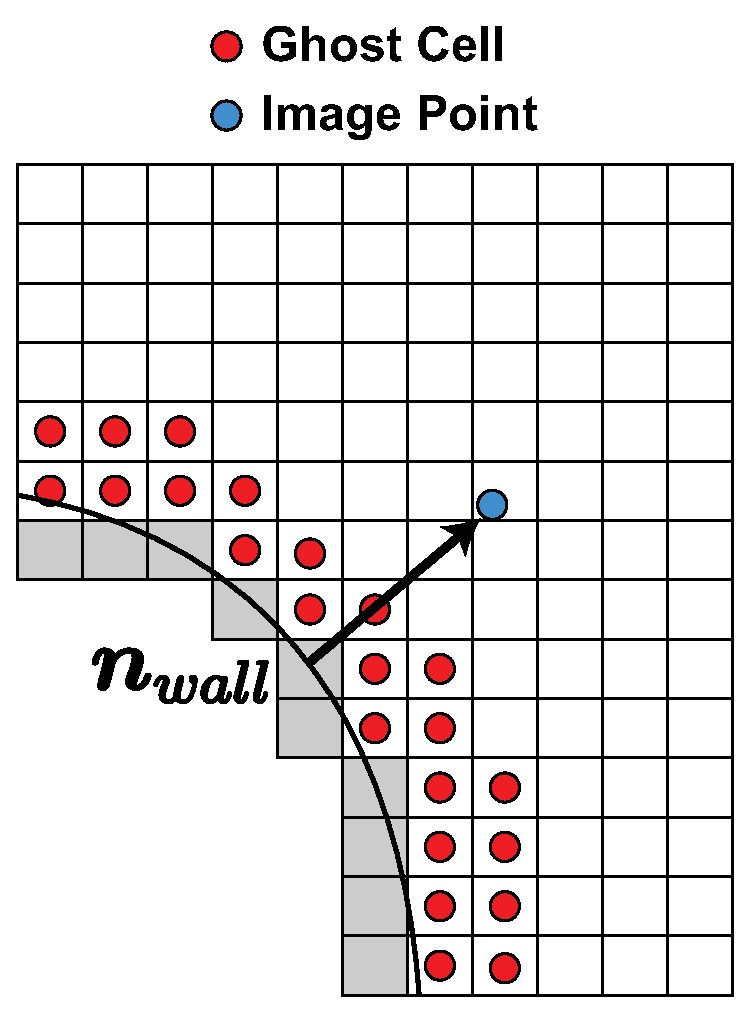
\includegraphics[trim={0cm 0cm 0cm 0cm},clip,width=0.35\textwidth]{FIGURES/IBM_ARTICLE/REGULAR_GC.eps}
    \label{ibm:fig:ghostCellRegular}%
    }
    \hspace*{0.2cm}
    \subfloat[Modified ghost-cell positioning at the prescribed distance $H_{\mathrm{mod}}$.]{%
    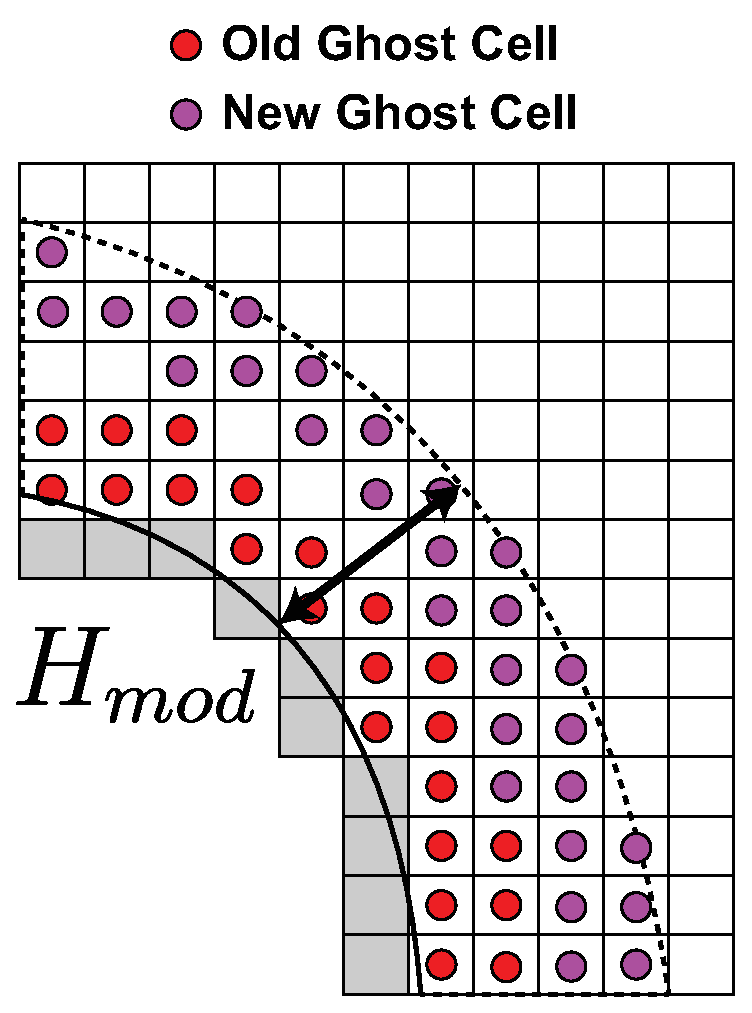
\includegraphics[trim={0cm 0cm 0cm 0cm},clip,width=0.35\textwidth]{FIGURES/IBM_ARTICLE/HMOD_GC.eps}
    \label{ibm:fig:ghostCellHmod}%
    }
    \caption{Schematic representation of the ghost-cell treatment near an immersed boundary. The standard approach (a) defines ghost-cell directly near the immerse-boundary, while the modified approach (b) adjusts the positioning of the ghost cells according to the prescribed modeling distance $H_{\mathrm{mod}}$ used for the RANS wall treatment.}
    \label{ibm:fig:ghostCells}
\end{figure}

In conventional body-fitted RANS simulations, the mesh is typically highly stretched in the wall-normal direction in order to resolve the large velocity gradients that develop inside the boundary layer. In an immersed-boundary framework, however, imposing a comparable near-wall spacing throughout the background mesh would be excessively restrictive, especially for the high-Reynolds-number conditions typical of aircraft icing simulations, and would substantially increase the overall computational cost. For this reason, wall functions are employed to relax the near-wall resolution requirement. Their application within the immersed-boundary framework, however, requires particular attention to the placement of the ghost cells and their associated image points. The standard ghost-cell construction presented earlier is not directly suitable for this purpose. When wall functions are used, the conventional positioning of target and image points does not guarantee that they lie within the same region of the boundary layer. This may lead to inconsistencies in the imposed wall-modeled boundary condition and produce spurious oscillations in the pressure and skin-friction coefficients.

% To address this issue, \cite{CONSTANT2021110240} proposed a modified ghost-cell placement strategy in which the location of the immersed-boundary target points is determined from a modeling height $H_{mod}$. This height is derived from flat-plate turbulent boundary-layer theory and is chosen so that the image points are located at an appropriate wall-modeling distance, while the target points define the modeled region below this threshold, as illustrated in Figure~\ref{ibm:fig:ghostCellHmod}. The modeling height is defined as
% \begin{equation}
%     H_{mod} = \sqrt{2} \frac{y_{target}^+ L}{Re \sqrt{0.058 Re^{-0.2}}}
%     \label{ibm:eq:hmod}
% \end{equation}
% where $y_{target}^+$ is the prescribed target wall coordinate, typically chosen in the logarithmic region of the boundary layer, with values between 50 and 300.

% The boundary conditions imposed at the ghost cell are then constructed from the corresponding image points. First, the pressure is assumed to remain constant in the wall-normal direction. Denoting the ghost cell by the subscript $GC$ and the image point by the subscript $IM$, this gives
% \begin{equation}
%     p_{GC} = p_{IM}
%     \label{ibm:eq:pressureGC}
% \end{equation}

% The imposed isothermal wall temperature is estimated from the freestream total temperature using the isentropic total-temperature relation
% \begin{equation}
%     \frac{T_0}{T_\infty} = 1 + \frac{1}{2}\left(\gamma - 1\right)M_\infty^2 
%     \label{ibm:eq:totalTemperatureRatio}
% \end{equation}
% where $T_0$ is the total temperature, $T_\infty$ is the freestream static temperature, $\gamma$ is the specific heat ratio, and $M_\infty$ is the freestream Mach number. The wall temperature is then prescribed as $T_w=T_0$. Rather than imposing this temperature directly at the ghost-cell center, the ghost-cell density is reconstructed from the image-point state as
% \begin{equation}
%     \rho_{GC} = 2\frac{p_{IM}}{R T_w} - \rho_{IM}
%     \label{ibm:eq:densityGC}
% \end{equation}

% \noindent The ghost-cell temperature is then obtained from the perfect-gas equation of state
% \begin{equation}
%     T_{GC} = \frac{p_{GC}}{R\rho_{GC}}
%     \label{ibm:eq:temperatureGC}
% \end{equation}
% where $R$ is the specific gas constant.

% The tangential velocity at the ghost cell is obtained from the selected wall law. A useful feature of the method is that the ghost-cell construction is independent of the particular wall function used. In the present chapter, the Reichardt \cite{prakash2019rans} wall function is adopted:
% \begin{equation}
%     u^+ = \frac{\ln\left(1 + \kappa y^+\right)}{\kappa} + 7.8 \left[1 - \exp\left(-\frac{y^+}{11}\right) - \frac{y^+}{11}\exp\left(-\frac{y^+}{3}\right)\right]
%     \label{ibm:eq:reichardt}
% \end{equation}
% where $\kappa \approx 0.41$ is the von Kármán constant.

% For the $k-\omega$ turbulence model, the ghost-cell values of the turbulent variables are also reconstructed from wall-function-consistent near-wall relations. The specific dissipation rate is obtained by blending its viscous-sublayer and logarithmic-layer asymptotic limits

% \begin{equation}
%     \omega_{\mathrm{vis}}
%     = \frac{6\nu_{GC}}{\beta_{\omega} y_{GC}^2},
%     \qquad
%     \omega_{\log}
%     = \frac{u_\tau}{\sqrt{C_\mu}\kappa y_{GC}},
%     \qquad
%     u_\tau = \sqrt{\frac{\tau_w}{\rho_{GC}}}.
%     \label{ibm:eq:omegaVisLogGC}
% \end{equation}

% where $\beta_{\omega} = 0.075$ and $C_\mu = 0.09$ are turbulence-model constants. The wall-function value imposed at the ghost cell is then defined as

% \begin{equation}
%     \omega_{GC} = \left(\omega_{\mathrm{vis}}^2+\omega_{\log}^2\right)^{1/2}
%     \label{ibm:eq:omegaGC}
% \end{equation}

% The turbulent kinetic energy is subsequently recovered from the eddy-viscosity relation

% \begin{equation}
%     \mu_t = \rho \frac{k}{\omega}
%     \qquad
%     k_{GC} = \frac{\mu_{t,GC}\omega_{GC}}{\rho_{GC}}
%     \label{ibm:eq:kGC}
% \end{equation}

% Although the cells located between the ghost-cell layer and the immersed geometry are not advanced by the flow solver, flow quantities are assigned to these cells at the end of the flow simulation using the same wall-function reconstruction. This additional reconstruction is required by the droplet impingement solver, which uses the near-wall flow field to evaluate droplet trajectories and surface impacts in the vicinity of the immersed boundary.

To address this issue, \cite{CONSTANT2021110240} proposed a modified ghost-cell placement strategy based on a modeling height $H_{mod}$. This height is estimated from a turbulent flat-plate skin-friction correlation and defines the near-wall region treated by the wall model. The ghost cells are consequently selected farther from the immersed boundary, immediately below the modeling height, while the corresponding image points lie approximately at $H_{mod}$, as illustrated in Figure~\ref{ibm:fig:ghostCellHmod}. The modeling height is defined as

\begin{equation}
    H_{mod} = \sqrt{2}\frac{y_{target}^+L}{Re_L\sqrt{0.058Re_L^{-0.2}}},
    \label{ibm:eq:hmod}
\end{equation}

where $L$ is the reference length, $Re_L$ is the corresponding freestream Reynolds number, and $y_{target}^+$ is the prescribed target wall coordinate, typically selected in the logarithmic region. A value of $y_{target}^+=100$ is adopted in the present work \cite{CONSTANT2021110240}.

The boundary conditions at each ghost cell are constructed from its corresponding image point. Denoting the ghost cell by the subscript $GC$ and the image point by the subscript $IM$, a zero wall-normal pressure gradient is imposed through

\begin{equation}
    p_{GC} = p_{IM}.
    \label{ibm:eq:pressureGC}
\end{equation}

An isothermal wall temperature $T_w$ is prescribed independently of the ghost-cell temperature. The wall density, friction velocity, and dimensionless wall coordinate are defined as

\begin{equation}
    \rho_w = \frac{p_{IM}}{RT_w},
    \qquad
    u_{\tau,w} = \sqrt{\frac{\tau_w}{\rho_w}},
    \qquad
    y^+ = \frac{\rho_wu_{\tau,w}y}{\mu_w},
    \label{ibm:eq:wallScaling}
\end{equation}

where $R$ is the specific gas constant, $\tau_w$ is the wall shear-stress magnitude, $\mu_w$ is the dynamic viscosity evaluated at $T_w$, and $y$ is the distance from the immersed wall.

The image-point velocity is decomposed into wall-normal and tangential components. The tangential velocity is reconstructed using the Reichardt wall law \cite{reichardt1956}, expressed as $u^+=f(y^+)$, where the friction velocity is determined iteratively from the image-point velocity:

\begin{equation}
    u_{t,IM} = u_{\tau,w}f(y_{IM}^+).
    \label{ibm:eq:imageVelocityWF}
\end{equation}

The ghost-cell velocity components are then prescribed as

\begin{equation}
    u_{t,GC} = u_{\tau,w}f(y_{GC}^+),
    \qquad
    u_{n,GC} = \frac{y_{GC}}{y_{IM}}u_{n,IM}.
    \label{ibm:eq:velocityGC}
\end{equation}

The temperature field is reconstructed using the Jayatilleke thermal wall function \cite{jayatilleke1969}, which relates the dimensionless temperature $T^+$ to the wall coordinate $y^+$. The temperature scale and ghost-cell temperature are obtained from

\begin{equation}
    T_\tau = \frac{T_w-T_{IM}}{T_{IM}^+},
    \qquad
    T_{GC} = T_w-T_{GC}^+T_\tau.
    \label{ibm:eq:temperatureGC}
\end{equation}

The ghost-cell density is subsequently recovered from the perfect-gas equation of state:

\begin{equation}
    \rho_{GC} = \frac{p_{IM}}{RT_{GC}}.
    \label{ibm:eq:densityGC}
\end{equation}

The wall heat flux and heat-transfer coefficient are evaluated as

\begin{equation}
    q_w = \frac{\rho_{IM}c_pu_{\tau,w}(T_w-T_{IM})}{T_{IM}^+},
    \qquad
    HTC = \frac{q_w}{T_w-T_{\mathrm{rec}}},
    \label{ibm:eq:heatTransferCoefficient}
\end{equation}

where $c_p$ is the specific heat at constant pressure and $T_{\mathrm{rec}}$ is the recovery temperature.

The $k$--$\omega$ turbulence model is employed in the present work. The ghost-cell turbulence variables are reconstructed using near-wall relations for the turbulent viscosity and specific dissipation rate, following the wall-function treatment of \cite{nichols2004wall}. The latter is obtained by blending the viscous-sublayer and logarithmic-layer contributions:

\begin{equation}
    \omega_{GC} = \sqrt{\omega_{\mathrm{vis}}^2+\omega_{\log}^2},
    \label{ibm:eq:omegaGC}
\end{equation}

where

\begin{equation}
    \omega_{\mathrm{vis}} = \frac{6\nu_{GC}}{\beta_\omega y_{GC}^2},
    \qquad
    \omega_{\log} = \frac{u_{\tau,GC}}{\sqrt{C_\mu}\kappa y_{GC}},
    \label{ibm:eq:omegaVisLogGC}
\end{equation}

with $\nu_{GC}=\mu_{GC}/\rho_{GC}$, $\beta_\omega=0.075$, $C_\mu=0.09$, $\kappa=0.41$, and $u_{\tau,GC}=\sqrt{\tau_w/\rho_{GC}}$. The turbulent kinetic energy is then reconstructed as

\begin{equation}
    k_{GC} = \frac{\mu_{t,GC}\omega_{GC}}{\rho_{GC}},
    \label{ibm:eq:kGC}
\end{equation}

where $\mu_{t,GC}$ is evaluated from the near-wall turbulent-viscosity relation. Wall roughness effects are also incorporated through corrections to the velocity and thermal wall functions, following \cite{chedevergne_aupoix} and \cite{prakash2019rans}, respectively. The details of these corrections are not presented here. These reconstructed near-wall flow quantities provide the velocity field required by the droplet impingement solver to evaluate trajectories and impacts near the immersed boundary.

\section{Immersed-Boundary Droplet Treatment}
\label{ibm:sec:dropSolver}

The Eulerian and Lagrangian droplet formulations used in \textsc{CHAMPS}, including their governing equations, trajectory integration, adaptive seeding, collection-efficiency evaluation, and SLD extensions, are described in the literature review (Sections~\ref{sec:eulerianTracking}--\ref{sec:review_sld}) and in Chapter~\ref{sec:lagArticle}. The present section is restricted to the modifications required to use both droplet formulations with an immersed geometry.

\subsection{Eulerian Formulation: Governing Equations and Penalization Strategy}
\label{ibm:sec:dropSolverEulerian}

% The governing continuity and momentum equations of the Eulerian droplet formulation are

% \begin{equation}
%     \frac{\partial \alpha}{\partial t}
%     + \nabla \cdot \left(\alpha \boldsymbol{u}_d\right) = 0
%     \label{ibm:eq:continuityDroplet}
% \end{equation}

% \begin{equation}
%     \frac{\partial \left(\alpha \boldsymbol{u}_d\right)}{\partial t}
%     + \nabla \cdot
%     \left(\alpha \boldsymbol{u}_d \otimes \boldsymbol{u}_d\right)
%     =
%     \frac{C_D Re_D}{24S_t}\alpha
%     \left(\boldsymbol{u}_a-\boldsymbol{u}_d\right)
%     +
%     \alpha
%     \left(1-\frac{\rho_a}{\rho_d}\right)
%     \frac{\boldsymbol{g}}{Fr^2},
%     \label{ibm:eq:momentumDroplet}
% \end{equation}
% where the variables and non-dimensional parameters are defined in Section~\ref{sec:eulerianTracking}.

% The immersed-boundary treatment follows the penalization strategy of \cite{lavoieDroplets}. 

The immersed-boundary treatment for the Eulerian droplet equations follows the penalization strategy of \cite{lavoieDroplets}. In this approach, source terms are introduced into the governing equations of the dispersed phase, presented in Section~\ref{sec:eulerianTracking}, to account for the presence of the immersed boundary. The penalization of these equations is enforced through the mask functions illustrated in Figure~\ref{ibm:fig:dropletPenalizationMasks}. The solid mask $\chi$, shown in Figure~\ref{ibm:fig:maskChi}, activates the penalization inside the immersed body:

\begin{equation}
    \chi =
    \begin{cases}
    1, & \phi \leq 0, \\
    0, & \phi > 0,
    \end{cases}
    \label{ibm:eq:solidMask}
\end{equation}

where negative values of $\phi$ correspond to the solid region and positive values to the fluid region. Since the penalization should be imposed only in the droplet shadow region, a second mask $\chi_d$, shown in Figure~\ref{ibm:fig:maskChiD}, is introduced:
\begin{equation}
    \chi_d =
    \begin{cases}
    1, & \boldsymbol{u}_d \cdot \boldsymbol{n}_{\phi} \leq 0, \\
    0, & \boldsymbol{u}_d \cdot \boldsymbol{n}_{\phi} > 0.
    \end{cases}
    \label{ibm:eq:dropletShadowMask}
\end{equation}

Thus, the penalization is active only where the immersed-solid and incoming-droplet regions overlap, through the combined mask $\chi\chi_d$, shown in Figure~\ref{ibm:fig:maskChiChiD}.

\begin{figure}[ht]
    \centering
    \subfloat[Solid--fluid mask $\chi$.]{%
    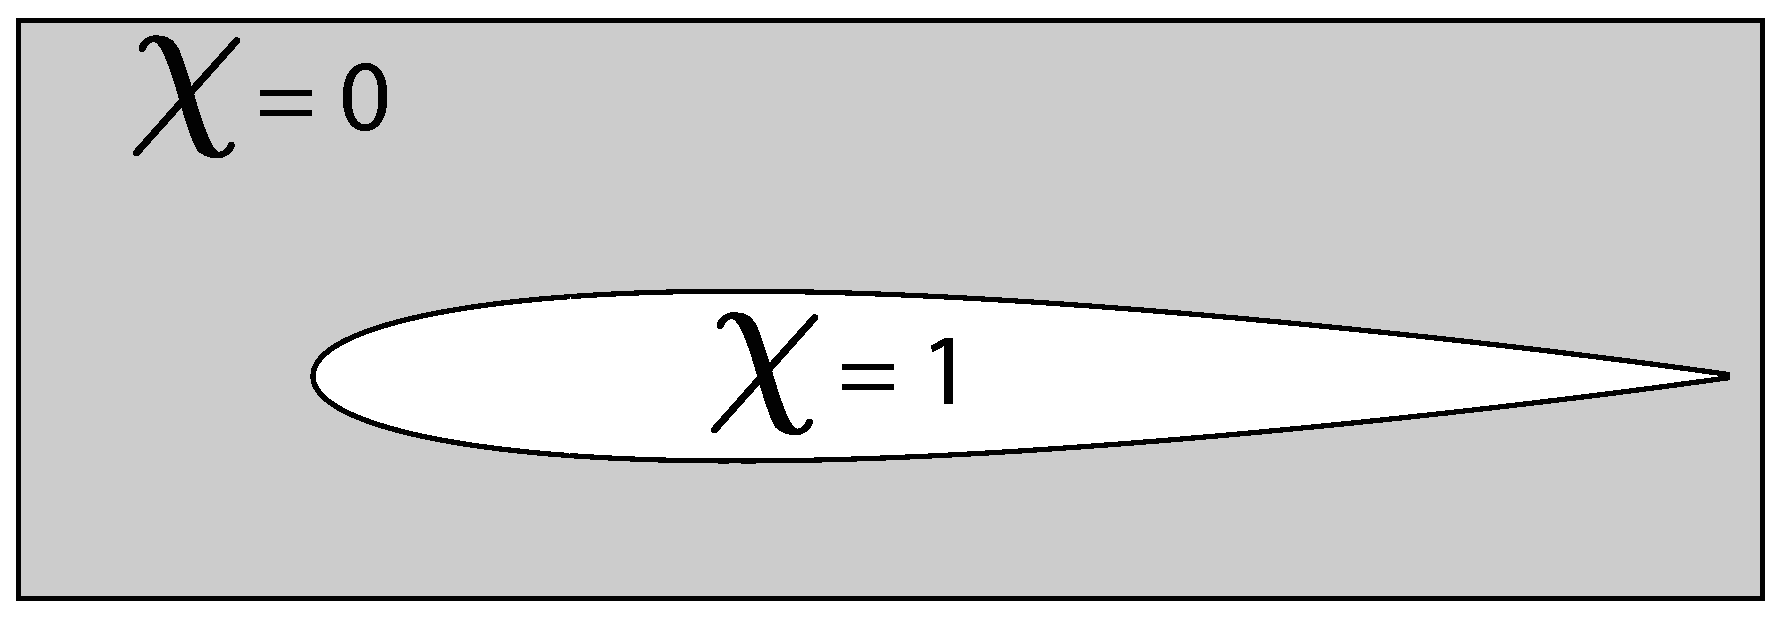
\includegraphics[trim={0cm 0cm 0cm 0cm},clip,width=0.5\textwidth]{FIGURES/IBM_ARTICLE/mask.eps}
    \label{ibm:fig:maskChi}%
    }
    \vspace*{0.3cm}
    \subfloat[Droplet-direction mask $\chi_d$.]{%
    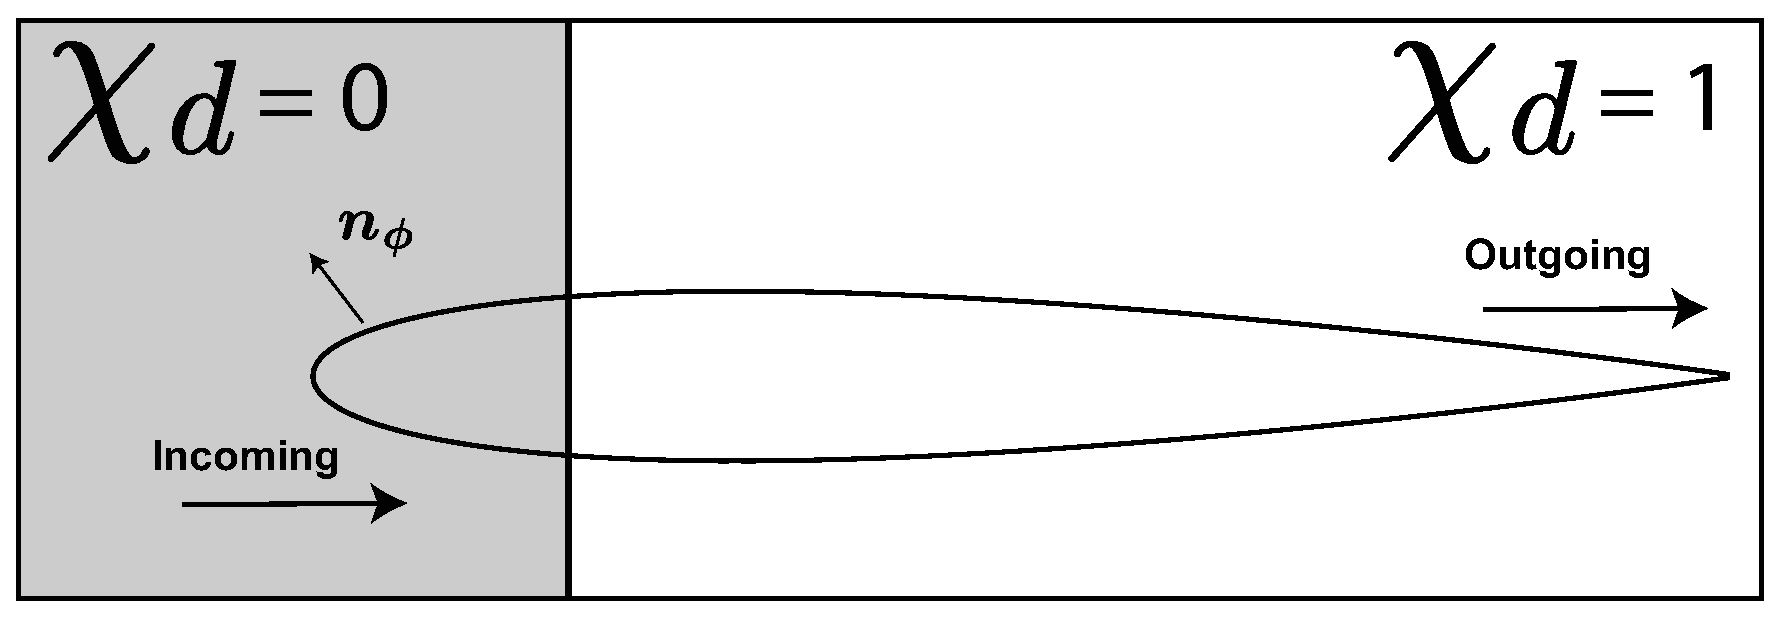
\includegraphics[trim={0cm 0cm 0cm 0cm},clip,width=0.5\textwidth]{FIGURES/IBM_ARTICLE/maskChiD.eps}
    \label{ibm:fig:maskChiD}%
    }
    \vspace*{0.3cm}
    \subfloat[Combined penalization indicator $\chi\chi_d$.]{%
    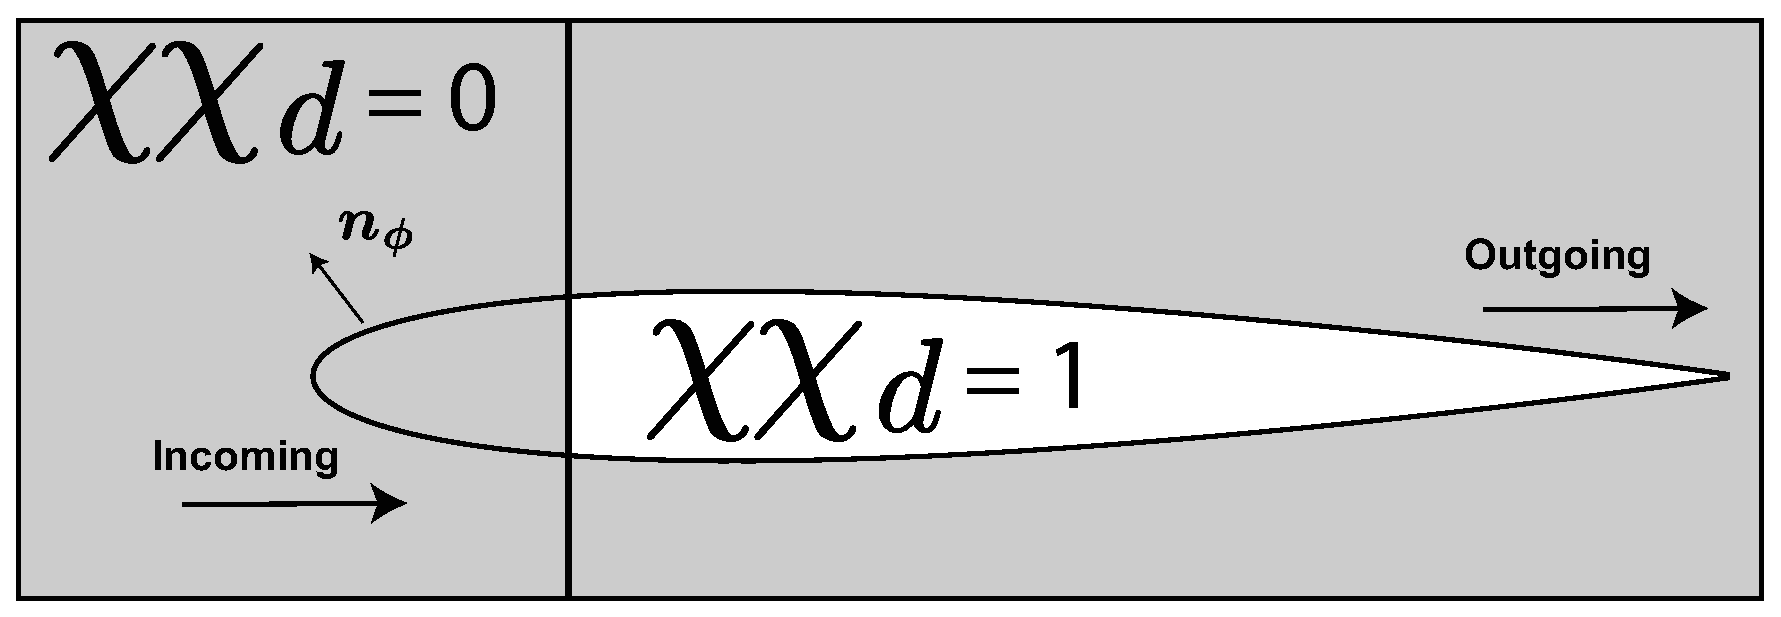
\includegraphics[trim={0cm 0cm 0cm 0cm},clip,width=0.5\textwidth]{FIGURES/IBM_ARTICLE/maskChiChiD.eps}
    \label{ibm:fig:maskChiChiD}%
    }
    \caption{Mask functions used in the penalized Eulerian droplet formulation: (a) solid--fluid mask $\chi$, (b) droplet-direction mask $\chi_d$, and (c) combined penalization indicator $\chi\chi_d$, which restricts the penalization to the overlap between the immersed-solid and incoming-droplet regions. \addText{Adapted from~\cite{lavoieDroplets}}.}
    \label{ibm:fig:dropletPenalizationMasks}
\end{figure}

The resulting penalized Eulerian droplet equations are
\begin{equation}
    \frac{\partial \alpha}{\partial t}
    + \nabla \cdot \left(\alpha \boldsymbol{u}_d\right)
    =
    -\frac{\chi\chi_d}{\eta}\alpha
    \label{ibm:eq:continuityDropletPenalized}
\end{equation}

{\small
\begin{equation}
\frac{\partial \left(\alpha \boldsymbol{u}_d\right)}{\partial t}
+ \nabla \cdot \left(\alpha \boldsymbol{u}_d \otimes \boldsymbol{u}_d\right)
=
\left(1-\chi\right)
\left[
\frac{C_D Re_D}{24S_t}\alpha\left(\boldsymbol{u}_a-\boldsymbol{u}_d\right)
+
\alpha\left(1-\frac{\rho_a}{\rho_d}\right)\frac{\boldsymbol{g}}{Fr^2}
\right]
-2\frac{\chi\chi_d}{\eta}\alpha\boldsymbol{u}_d
\label{ibm:eq:momentumDropletPenalized}
\end{equation}}

where $\eta$ controls the penalization strength and is set to $10^{-8}$. In the fluid region, where $\chi=0$, the penalization terms vanish and the original governing equations are recovered. In the penalized region, where $\chi\chi_d=1$, the source terms drive both the droplet volume fraction and momentum toward zero, corresponding to the immersed-boundary analogue of imposing a Dirichlet condition for the droplet phase.

\subsection{Lagrangian Immersed-Surface Tracking}
\label{ibm:sec:dropSolverLagrangian}

In a body-fitted formulation, droplet impacts are detected directly on boundary faces. In an immersed-boundary framework, however, the solid surface is not a boundary of the volume mesh, and a dedicated impact treatment is therefore required. The Lagrangian tracking algorithm presented in Chapter~\ref{sec:lagArticle} remains unchanged; only the treatment used to detect and locate impacts on the immersed surface is modified. During preprocessing, cells intersected by the immersed geometry are tagged as potential impact cells and linked to the corresponding immersed-surface elements. This restricts the impact search during tracking to a local subset of surface elements.

\begin{figure}[htbp]
    \centering
    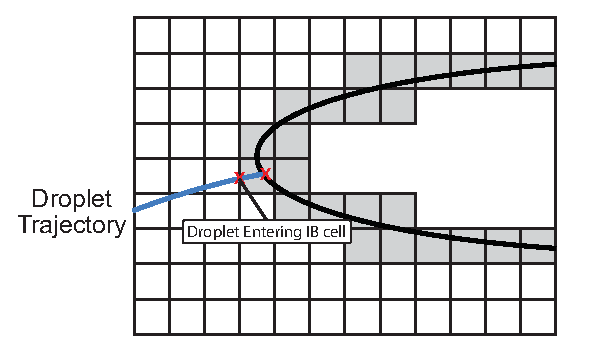
\includegraphics[trim={0cm 0cm 0cm 0cm},clip,width=0.6\textwidth]{FIGURES/IBM_ARTICLE/surfaceIntersection.eps}
    \caption{Droplet tracking in an immersed-boundary framework. The trajectory is advanced through the background mesh until it intersects the reconstructed immersed surface.}
    \label{ibm:fig:dropletTrajectories}
\end{figure}

Droplets are seeded upstream and advanced through regular fluid cells using the volume-mesh connectivity. When the next crossed cell is tagged as an immersed-boundary cell, the trajectory ray is tested against the associated surface elements to determine the physical impact location, as illustrated in Figure~\ref{ibm:fig:dropletTrajectories}. The local collection efficiency is then evaluated from the deformation of the droplet streamtube surrounding each impacting droplet using the methodology presented in Chapter~\ref{sec:lagArticle}. The SLD models require no modification for the immersed-boundary formulation, since droplet deformation is accounted for through the drag formulation and splashing is applied as a post-impact treatment. Only the splashing model of Wright et al.~\cite{wright2004semi} is considered in the present chapter for both the Eulerian and Lagrangian simulations.

\section{Immersed-Boundary Icing Coupling}
\label{ibm:sec:thermoGeo}

For each accretion layer, the RANS and droplet solutions are first obtained on the non-conformal background mesh. The aerodynamic and droplet quantities required by the thermodynamic calculation are then evaluated at the physical immersed surface. The thermodynamic solver, based on the iterative Messinger method, determines the local ice-growth distribution, which is subsequently transferred to the adapted level-set mesh. The ice--air interface is advanced using the continuous level-set methodology presented in Chapter~\ref{sec:lsArticle}, and the newly extracted ice surface replaces the previous immersed geometry. The signed-distance field and the immersed-boundary masks are then recomputed to account for the updated geometry, and the flow and droplet solutions are recalculated on the same background mesh for the following accretion layer.

The resulting multilayer procedure is hybrid with respect to the computational meshes. The RANS and droplet solvers retain the non-conformal background mesh as the ice geometry evolves, while the level-set calculation uses a separate Delaunay mesh composed of simplicial tetrahedral elements for interface evolution. Unlike a body-fitted RANS mesh, the level-set mesh does not require the stringent near-wall first-cell spacing or boundary-layer refinement imposed by the aerodynamic calculation. It can therefore be generated comparatively easily and at low computational cost as the ice geometry evolves.

\section{Results}
\label{ibm:sec:results}

The objective of this section is to assess the droplet impingement and icing capabilities of \textsc{CHAMPS} in an immersed-boundary setting. Both Eulerian and Lagrangian droplet formulations are considered, with and without supercooled-large-droplet (SLD) effects. A canonical cylinder case is first used for verification. The second case corresponds to the SLD impingement experiment of \cite{papadakism2004water}, which is used to evaluate the SLD effects on the predicted collection efficiency. Two NACA~0012 icing cases from wind-tunnel experiments \cite{trontin2017description} are then considered to assess the complete icing framework under rime and glaze conditions. Finally, the RG15 configuration considered during IPW2 is used as a demonstration of the complete immersed-boundary multilayer framework in 3D. The immersed-boundary background meshes used for these cases were generated using the quadtree meshing library developed by \cite{jaillet2022quadtree}.

\begin{table}[ht]
\centering
\caption{Summary of the benchmark cases.}
\begin{tabular}{cccc}
\hline \hline
Parameter & SLD & 001 & 004\\
\hline
Geometry & \makecell{2D NACA 23012} & \makecell{2D NACA 0012} & \makecell{2D NACA 0012} \\
Icing time [$s$] & N/A & 420 & 384.0 \\
LWC [$g/m^3$] & 0.5 & 0.6 & 0.55 \\
MVD [$\mu m$] & 111.0 & 20.0 & 15.0 \\
Ma [-] & 0.232 & 0.325 & 0.317 \\
AOA [\textdegree] & 2.5 & 4.0 & 4.0 \\
$C_{\mathrm{ref}}$ [inch] & 36 & 36 & 21 \\
$T_{\mathrm{static}}$ [$K$] & 268.02 & 250.7 & 262.3 \\
Re [-] & $4.57 \cdot 10^6$ & $4.83 \cdot 10^6$ & $4.44 \cdot 10^6$\\
\hline \hline
\end{tabular}
\label{ibm:tab:results}
\end{table}

\subsection{Cylinder Impingement Verification}
\label{ibm:sec:cylinder}

The cylinder case is used as a verification benchmark for the droplet impingement solvers. With drag and gravity neglected, droplets follow straight trajectories before impact, yielding an analytical solution for the collection efficiency \cite{lavoieDroplets}. For a cylinder of radius $R$ centered at the origin and an incoming droplet velocity aligned with the $x$ direction, the analytical solution can be written along the cylinder surface as

\begin{equation}
    \beta_{\mathrm{ana}} = \alpha_{\infty} U_{\infty} \max\left(-\cos\theta,0\right)
    \label{ibm:eq:cylinderAnalyticalBeta}
\end{equation}

where $\theta$ is the polar angle along the cylinder surface and $\alpha_{\infty}$ is the freestream droplet volume fraction. In the present verification case, $\alpha_{\infty}$ and $U_{\infty}$ are both set to unity, so the analytical collection efficiency reaches its maximum value $\beta_{\mathrm{ana}}=1$ at $\theta=\pi$, decreases to zero at $\theta=\pi\pm\pi/2$, and remains zero over the rear side of the cylinder.

\begin{figure}[ht!]
    \centering
    \subfloat[Eulerian body-fitted.]{%
    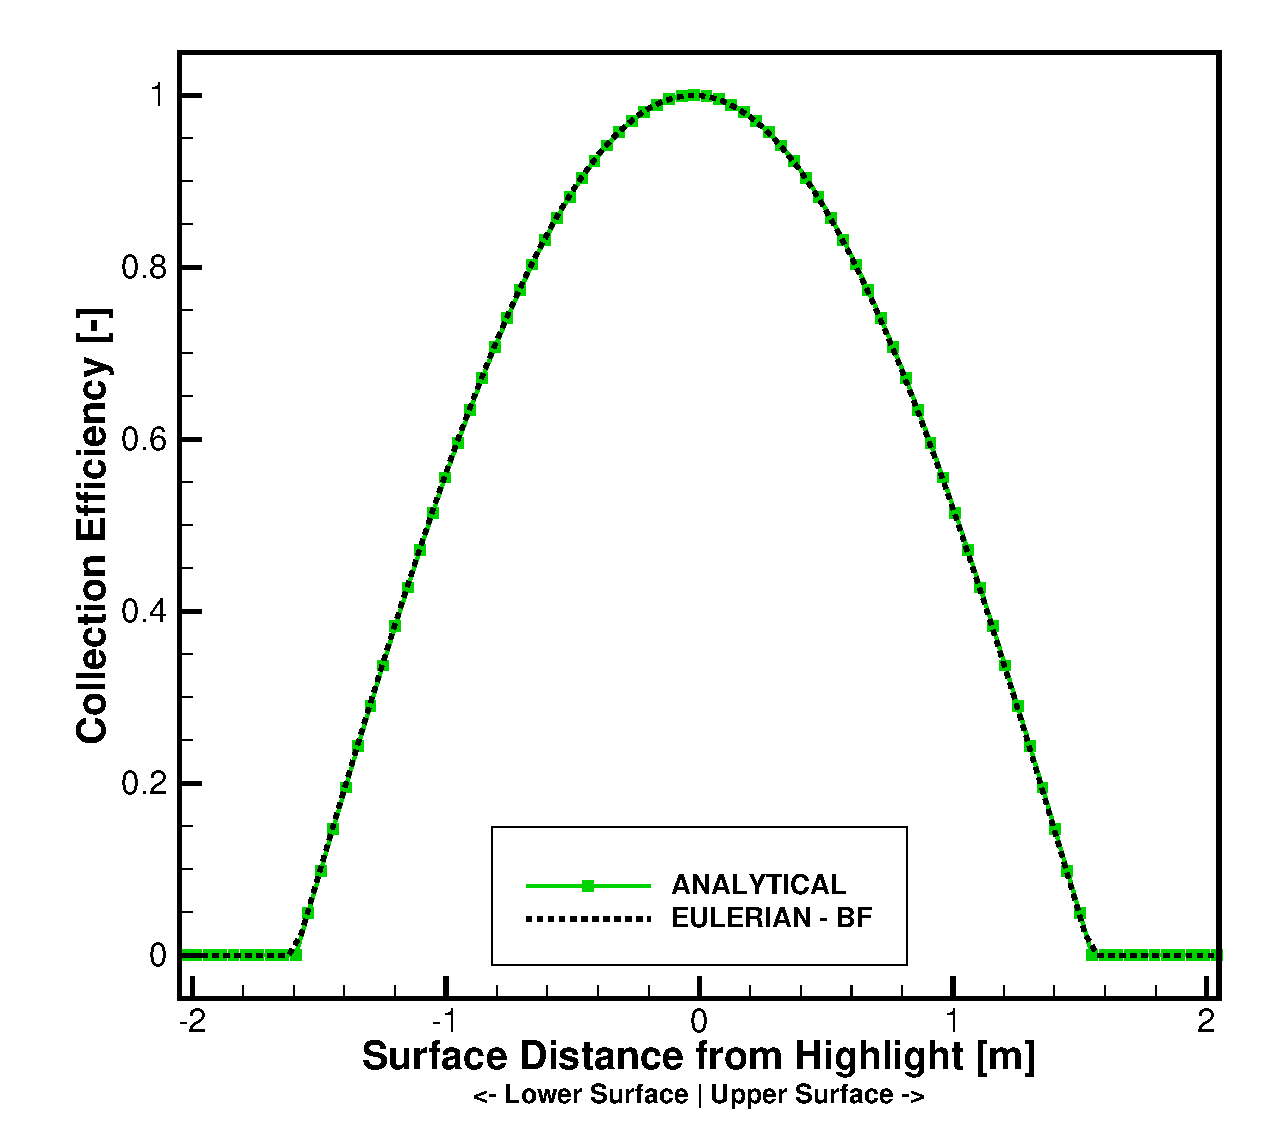
\includegraphics[trim={0cm 0cm 0cm 0cm},clip,width=0.4\textwidth]{FIGURES/IBM_ARTICLE/CASE_CYLINDER_EUL_BF_BETA.eps}
    \label{ibm:fig:cylinderEulerianBFBETA}%
    }
    \subfloat[Eulerian immersed-boundary.]{%
    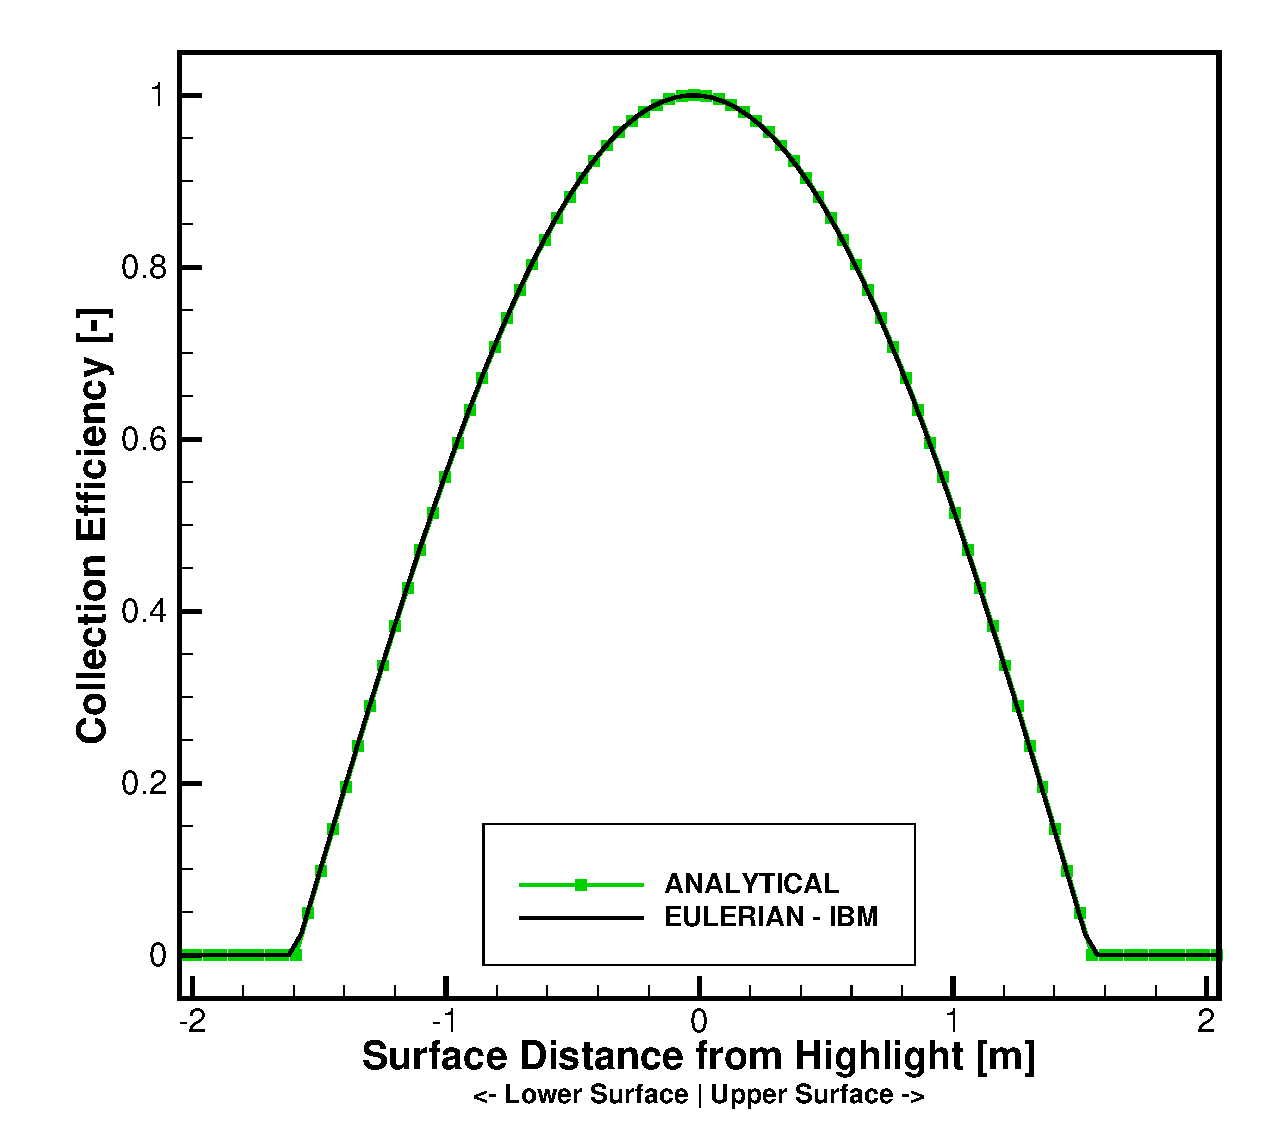
\includegraphics[trim={0cm 0cm 0cm 0cm},clip,width=0.4\textwidth]{FIGURES/IBM_ARTICLE/CASE_CYLINDER_EUL_IBM_BETA.eps}
    \label{ibm:fig:cylinderEulerianIBMBETA}%
    }

    \subfloat[Lagrangian body-fitted.]{%
    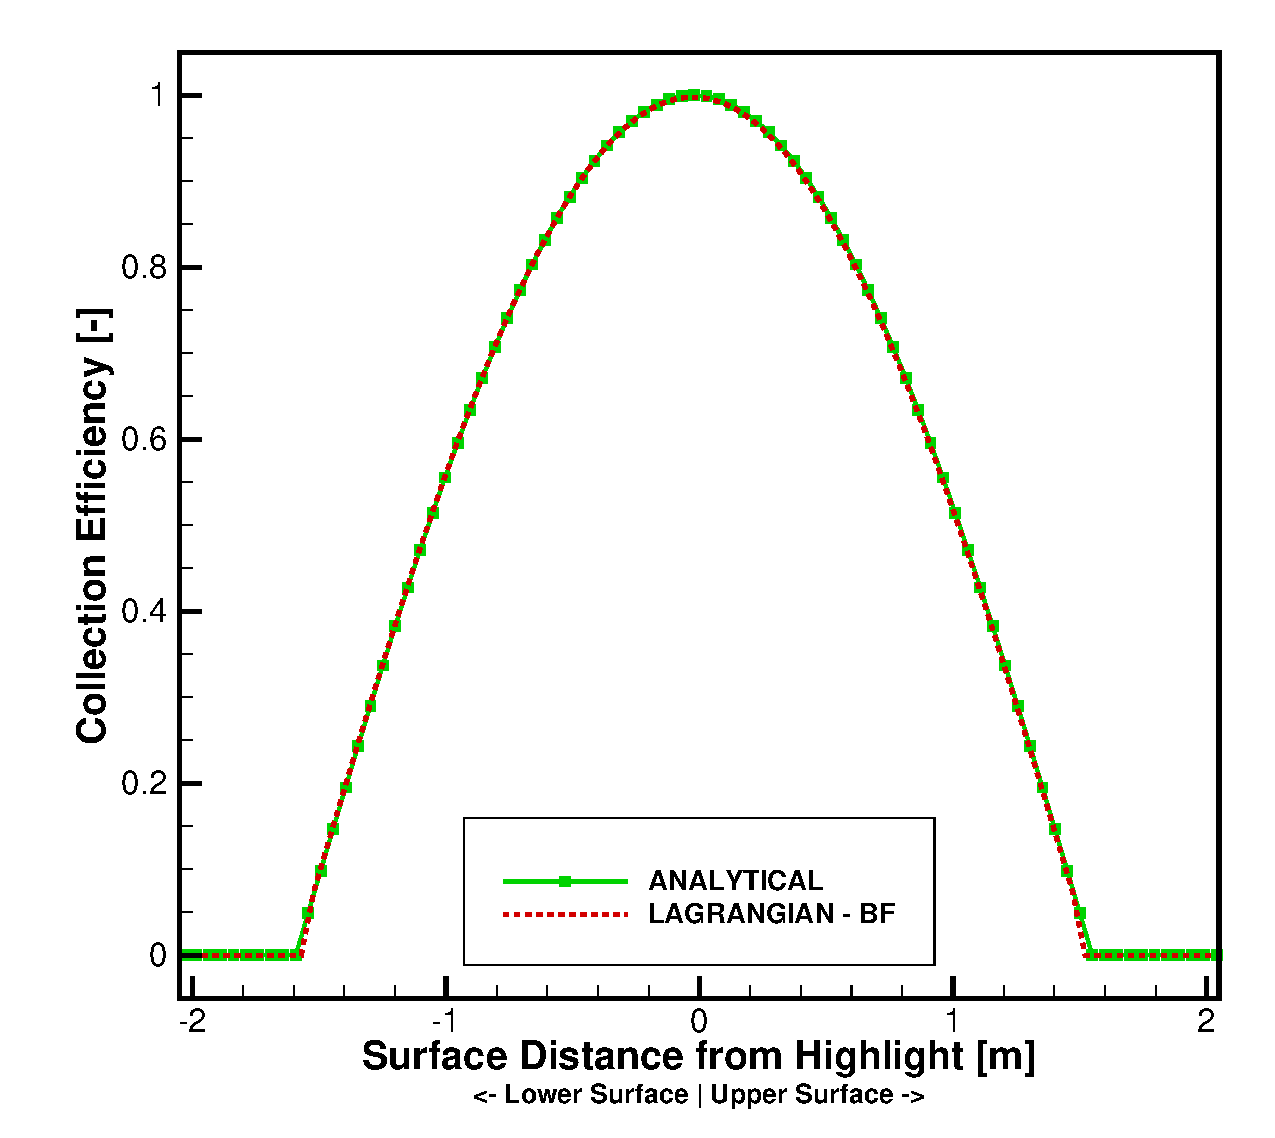
\includegraphics[trim={0cm 0cm 0cm 0cm},clip,width=0.4\textwidth]{FIGURES/IBM_ARTICLE/CASE_CYLINDER_LAG_BF_BETA.eps}
    \label{ibm:fig:cylinderLagrangianBFBETA}%
    }
    \subfloat[Lagrangian immersed-boundary.]{%
    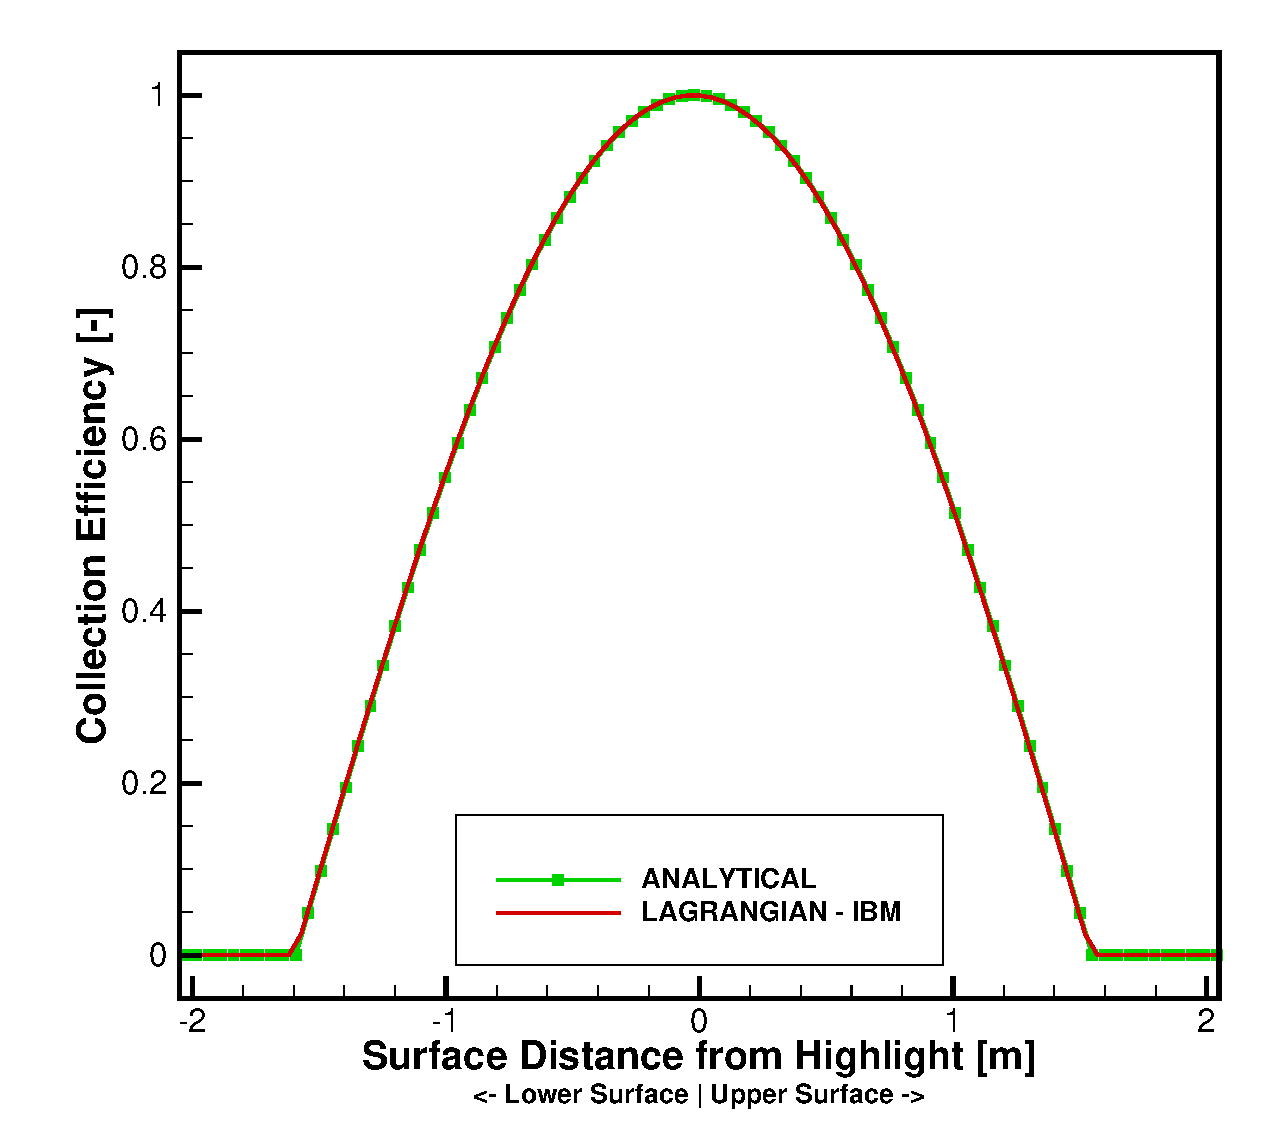
\includegraphics[trim={0cm 0cm 0cm 0cm},clip,width=0.4\textwidth]{FIGURES/IBM_ARTICLE/CASE_CYLINDER_LAG_IBM_BETA.eps}
    \label{ibm:fig:cylinderLagrangianIBMBETA}%
    }
    \caption{Collection efficiency distributions on the cylinder obtained with Eulerian and Lagrangian formulations on body-fitted and immersed-boundary meshes.}
    \label{ibm:fig:cylinderBETA}
\end{figure}

Figure~\ref{ibm:fig:cylinderBETA} compares the Eulerian and Lagrangian predictions on both body-fitted and immersed-boundary meshes. All approaches reproduce the analytical solution, confirming the correctness of the droplet transport and impact detection procedures.

\subsection{SLD Impingement}
\label{ibm:sec:impingementSLD}

The NACA~23012 benchmark of \cite{papadakism2004water} is considered to evaluate the SLD modelling. This experiment provides collection efficiency measurements for large droplets and highlights the limitations of conventional trajectory models when droplet splashing is neglected. In particular, simulations without SLD effects generally overpredict both the magnitude and the extent of water collection.

The collection efficiency distributions are shown in Figure~\ref{ibm:fig:sldBETA}. For both Eulerian and Lagrangian formulations, the baseline predictions without SLD effects overestimate the experimental data, especially away from the stagnation region. When the SLD model is activated, splashing removes part of the impacting water mass, reducing the deposited collection efficiency and improving agreement with the experimental measurements. The body-fitted and immersed-boundary formulations show similar responses to the SLD correction, confirming the consistency of the immersed-boundary implementation.

\begin{figure}[ht!]
    \centering
    \subfloat[Eulerian formulation.]{%
    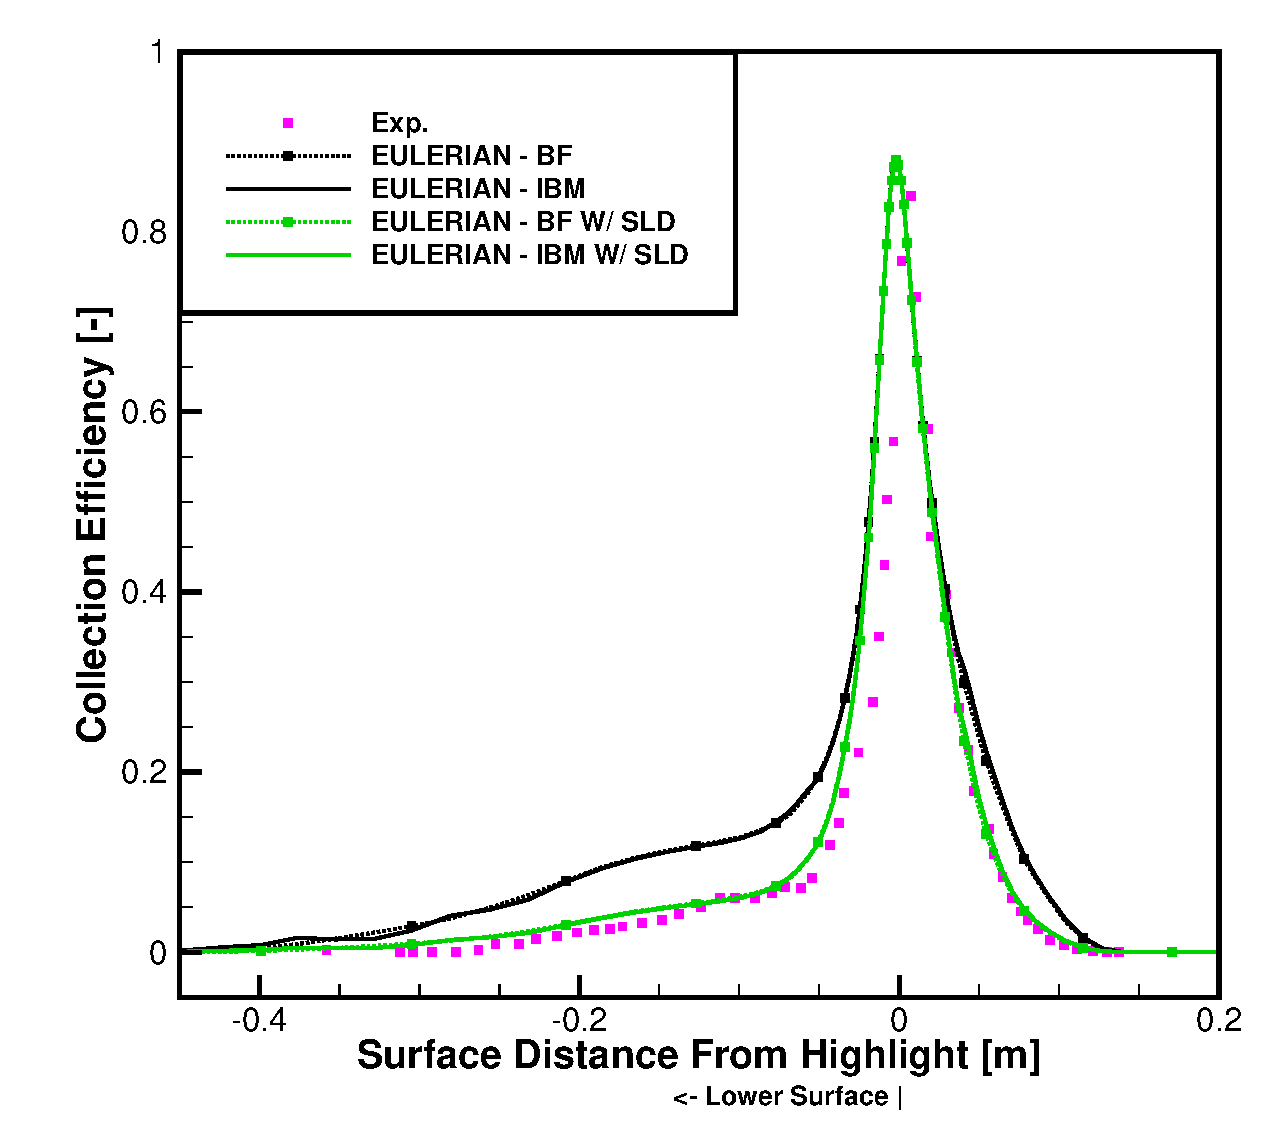
\includegraphics[trim={0cm 0cm 0cm 0cm},clip,width=0.49\textwidth]{FIGURES/IBM_ARTICLE/CASE_SLD_EULERIAN_BETA.eps}
    \label{ibm:fig:sldEulerianBETA}%
    }
    \subfloat[Lagrangian formulation.]{%
    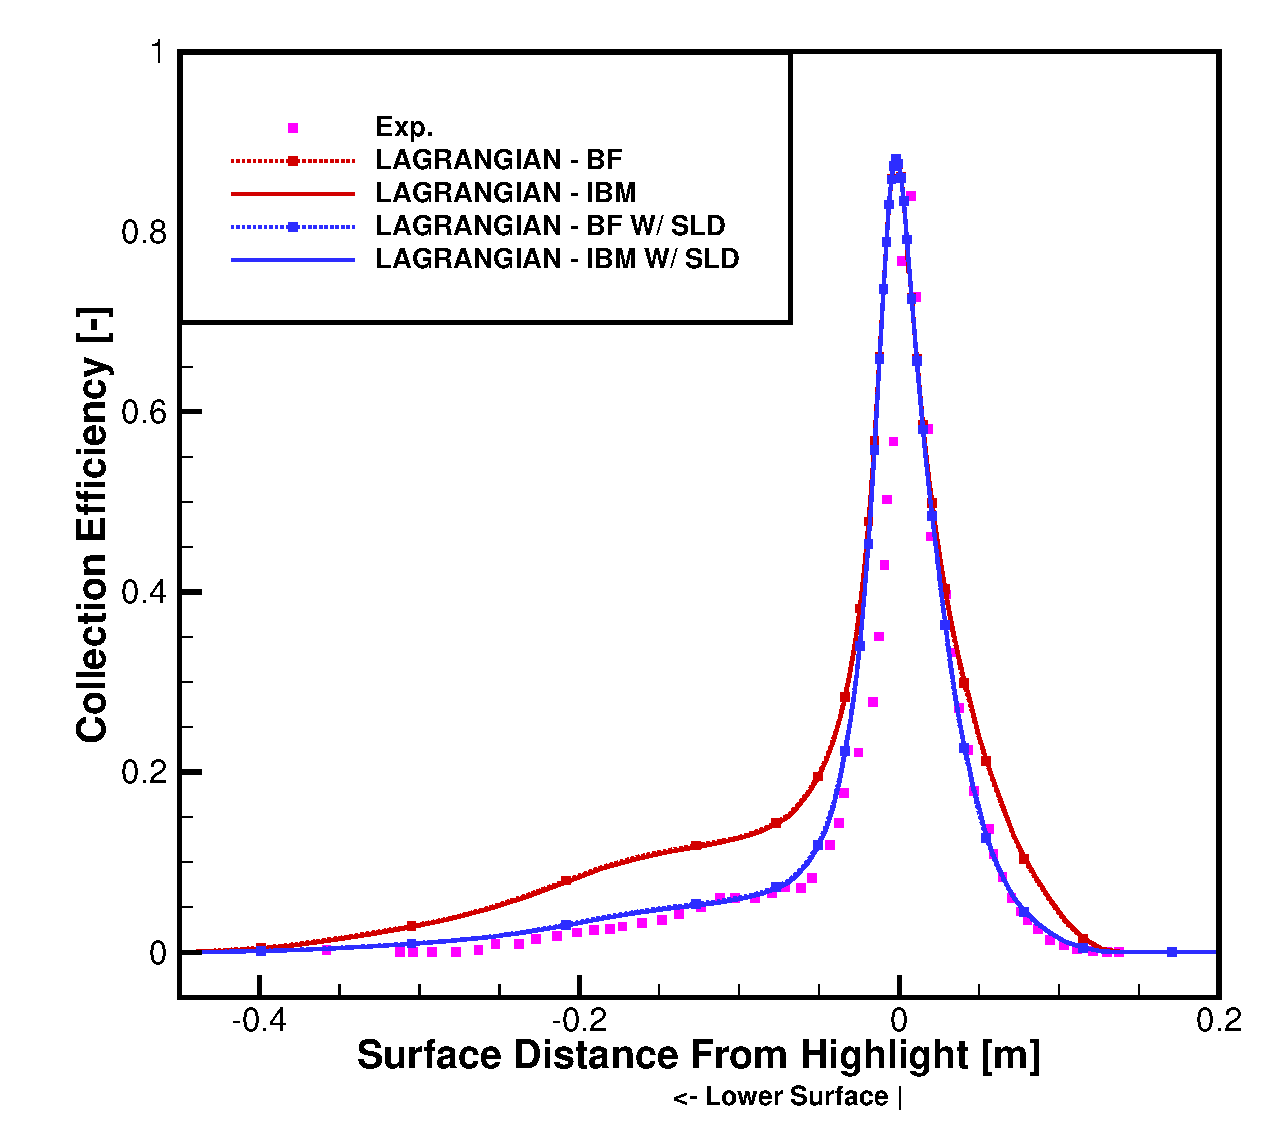
\includegraphics[trim={0cm 0cm 0cm 0cm},clip,width=0.49\textwidth]{FIGURES/IBM_ARTICLE/CASE_SLD_LAGRANGIAN_BETA.eps}
    \label{ibm:fig:sldLagrangianBETA}%
    }
    \caption{Collection efficiency distributions for the SLD impingement case \cite{papadakism2004water} obtained with the Eulerian and Lagrangian formulations, with and without SLD effects.}
    \label{ibm:fig:sldBETA}
\end{figure}

Some discrepancies remain near the stagnation region, where the peak collection efficiency is overpredicted. This behavior is consistent with the Wright et al. splashing model~\cite{wright2004semi}, which assumes limited mass loss for normal impacts, while splashing becomes more important farther from the stagnation point as the impact angle becomes more tangential to the surface. Since both formulations yield similar results, only the Lagrangian formulation is retained for the remainder of this section due to its computational efficiency for such cases.

\subsection{Case 01}
\label{ibm:sec:case01}

Case~01 corresponds to a rime ice condition, where droplets freeze upon impact. Under these conditions, water runback is negligible and the ice shape is mainly governed by the collection efficiency distribution. Since the impingement verification showed close agreement between body-fitted and immersed-boundary methods, similar ice shapes are expected.

\begin{figure}[ht]
    \centering
    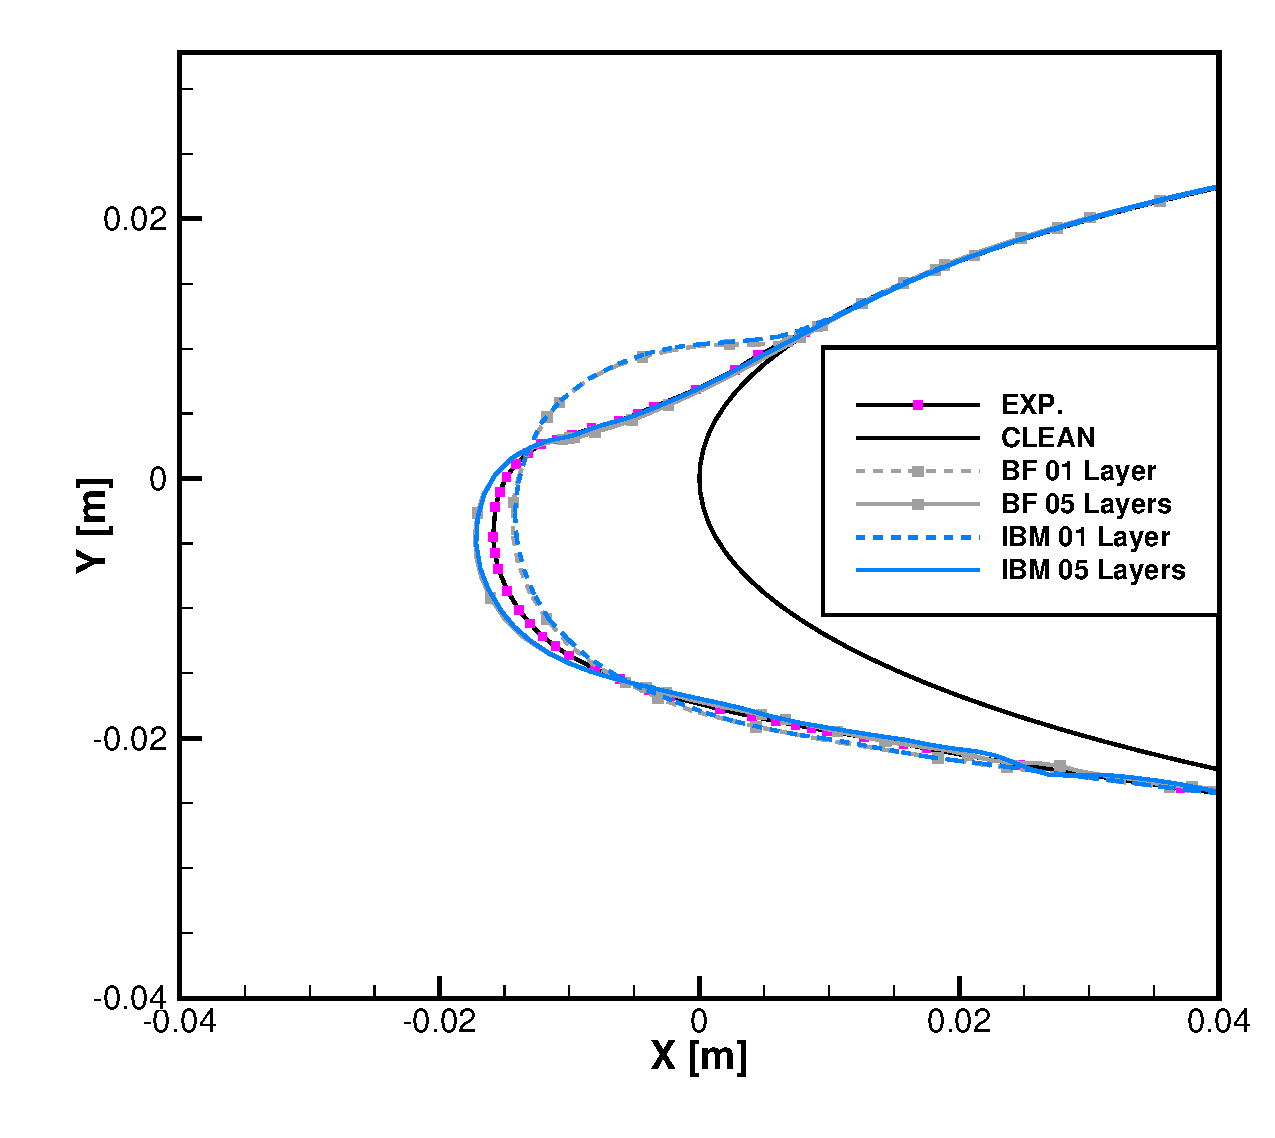
\includegraphics[trim={.1cm .1cm .1cm .1cm},clip,width=0.75\textwidth]{FIGURES/IBM_ARTICLE/CASE_01_ICE_SHAPE.eps}
    \caption{Predicted ice shapes for Case~01 using body-fitted and immersed-boundary formulations. The clean and experimental profiles are shown for reference, together with predictions obtained using 1 and 5 accretion layers.}
    \label{ibm:fig:Case01IceShape}
\end{figure}

The predicted ice shapes are shown in Figure~\ref{ibm:fig:Case01IceShape}. The body-fitted and immersed-boundary results are in good agreement for both single-layer and multilayer simulations. The five-layer prediction shows improved agreement with the experimental profile compared with the single-layer result. This supports the point discussed earlier in Section~\ref{ibm:sec:introduction}: updating the flow, droplet, thermodynamic, and geometric fields over successive accretion steps provides a more accurate representation of the evolving ice shape than a single-step calculation. The overall agreement with the experimental data confirms that the immersed-boundary framework is able to reproduce impingement-driven rime ice accretion with good accuracy.

\subsection{Case 04}
\label{ibm:sec:case04}

Case~04 corresponds to a glaze ice condition, where only part of the collected water freezes locally, while the remaining liquid forms a water film that runs back along the surface and progressively freezes downstream. The ice shape therefore depends not only on droplet impingement, but also on the local thermodynamic balance and convective heat transfer. Compared with rime ice, glaze ice prediction is therefore more sensitive to the wall treatment.

The predicted ice shapes and the corresponding heat transfer coefficient distributions are presented in Figure~\ref{ibm:fig:case04IceShapeHTC}. Although the same wall-function formulation is used, differences in the enforcement of the wall boundary condition lead to variations in the predicted heat transfer coefficient. The immersed-boundary solution predicts slightly larger heat transfer near the leading edge, where glaze ice growth is particularly sensitive to thermal effects.

\begin{figure}[ht!]
    \centering
    \subfloat[Single-layer ice shape.]{%
    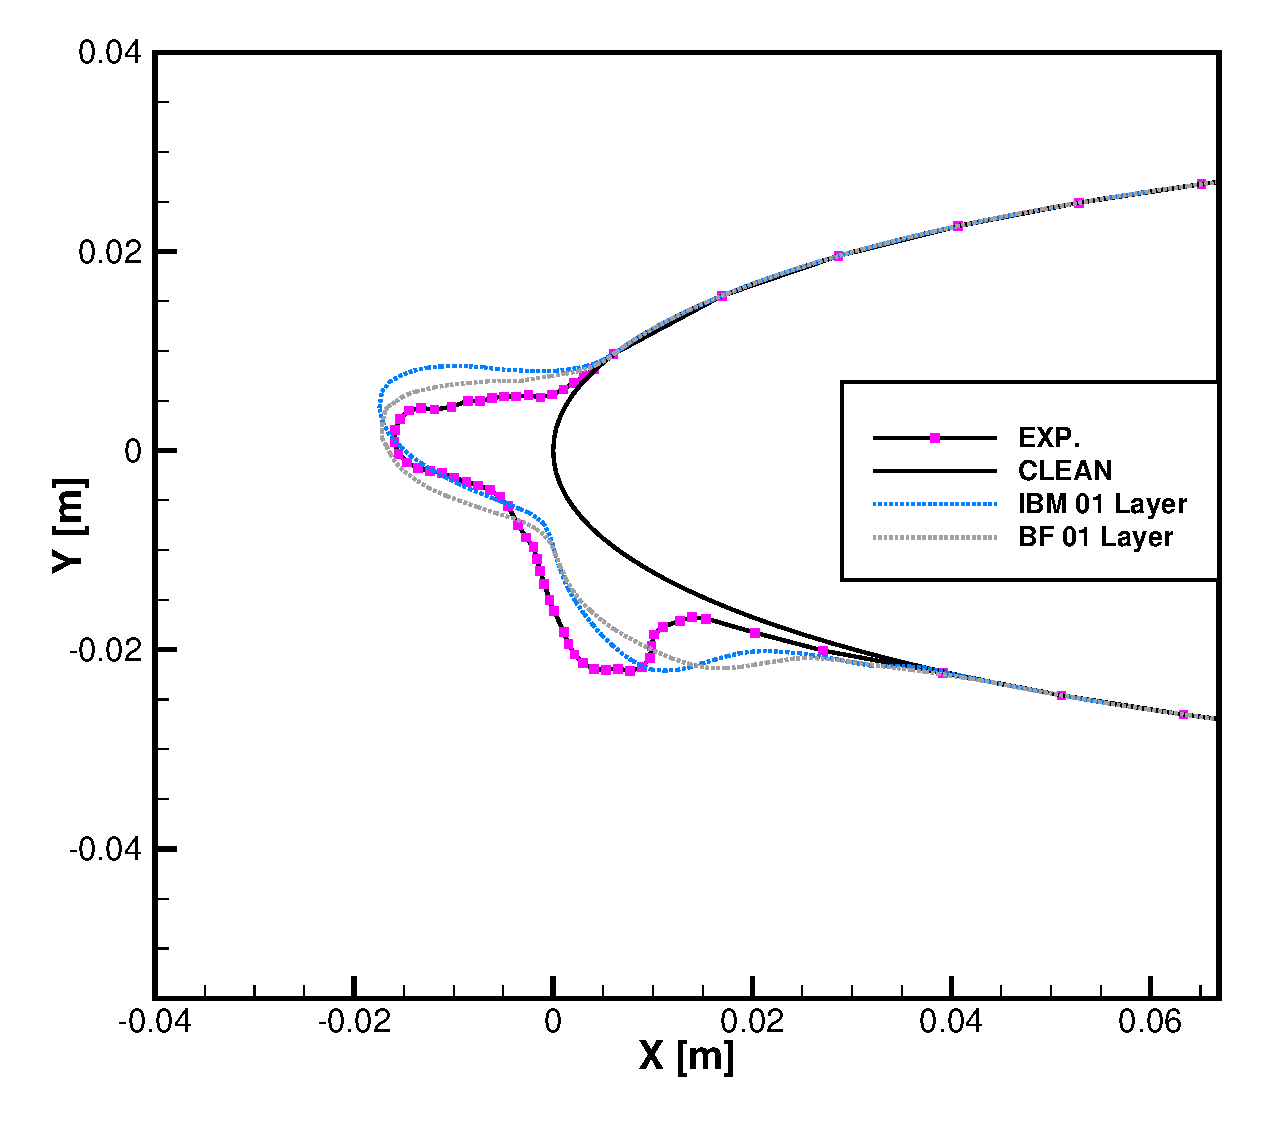
\includegraphics[trim={0cm 0cm 0cm 0cm},clip,width=0.49\textwidth]{FIGURES/IBM_ARTICLE/CASE_04_ICE_SHAPE_01_LAYER.eps}
    \label{ibm:fig:Case04IceShape1Layer}%
    }
    \subfloat[Five-layer ice shape.]{%
    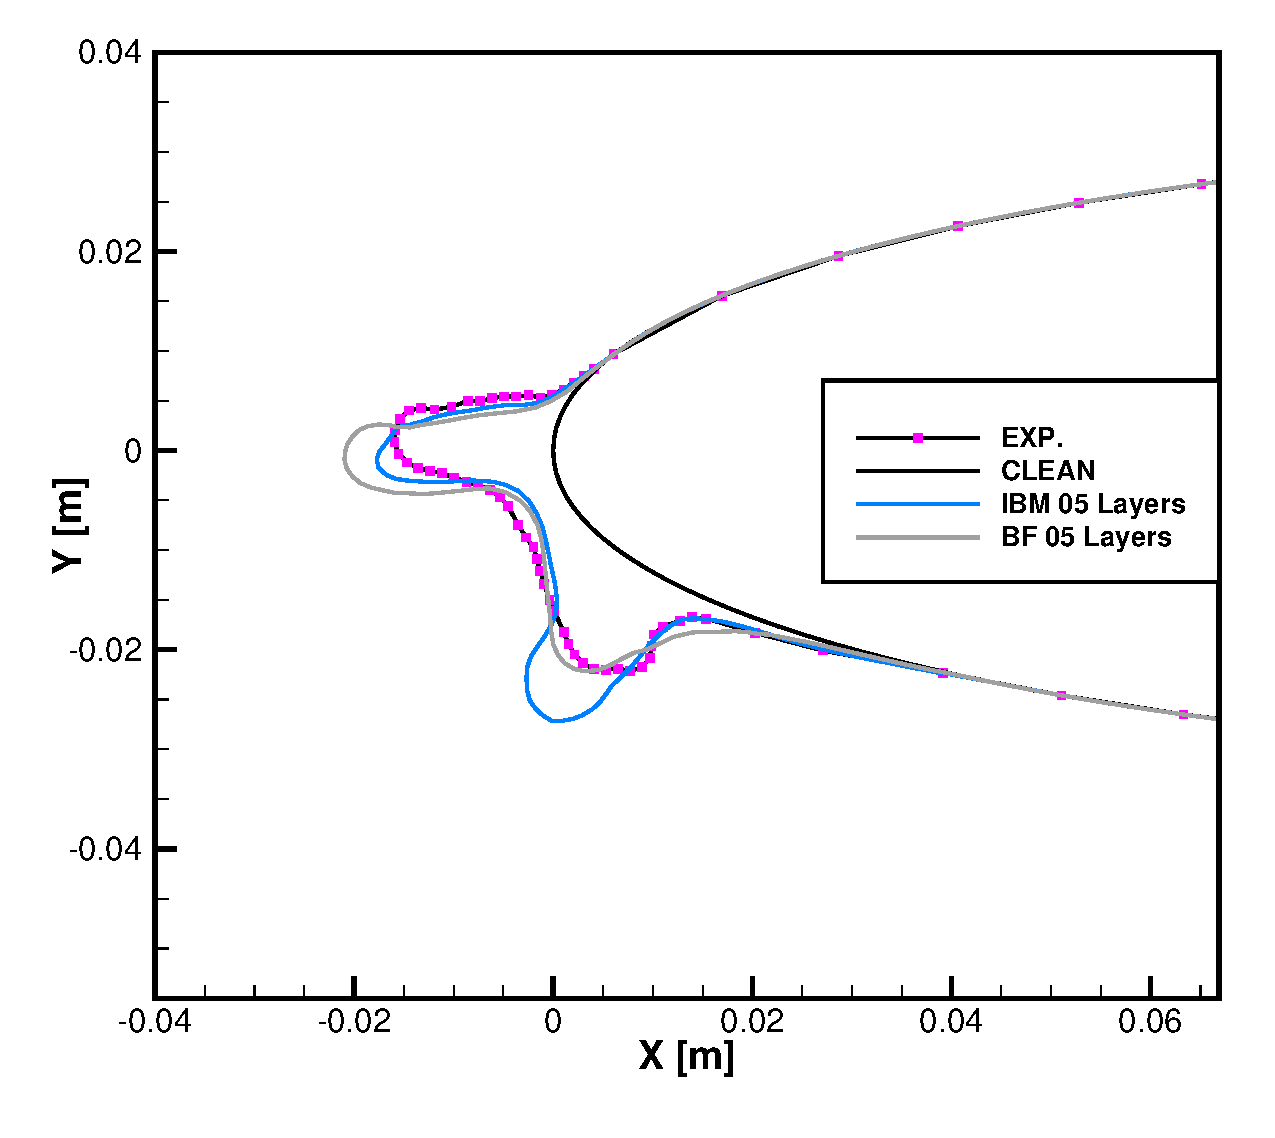
\includegraphics[trim={0cm 0cm 0cm 0cm},clip,width=0.49\textwidth]{FIGURES/IBM_ARTICLE/CASE_04_ICE_SHAPE_05_LAYER.eps}
    \label{ibm:fig:Case04IceShape5Layers}%
    }
    \vspace{0.2cm}
    \subfloat[Convective heat transfer coefficient.]{%
    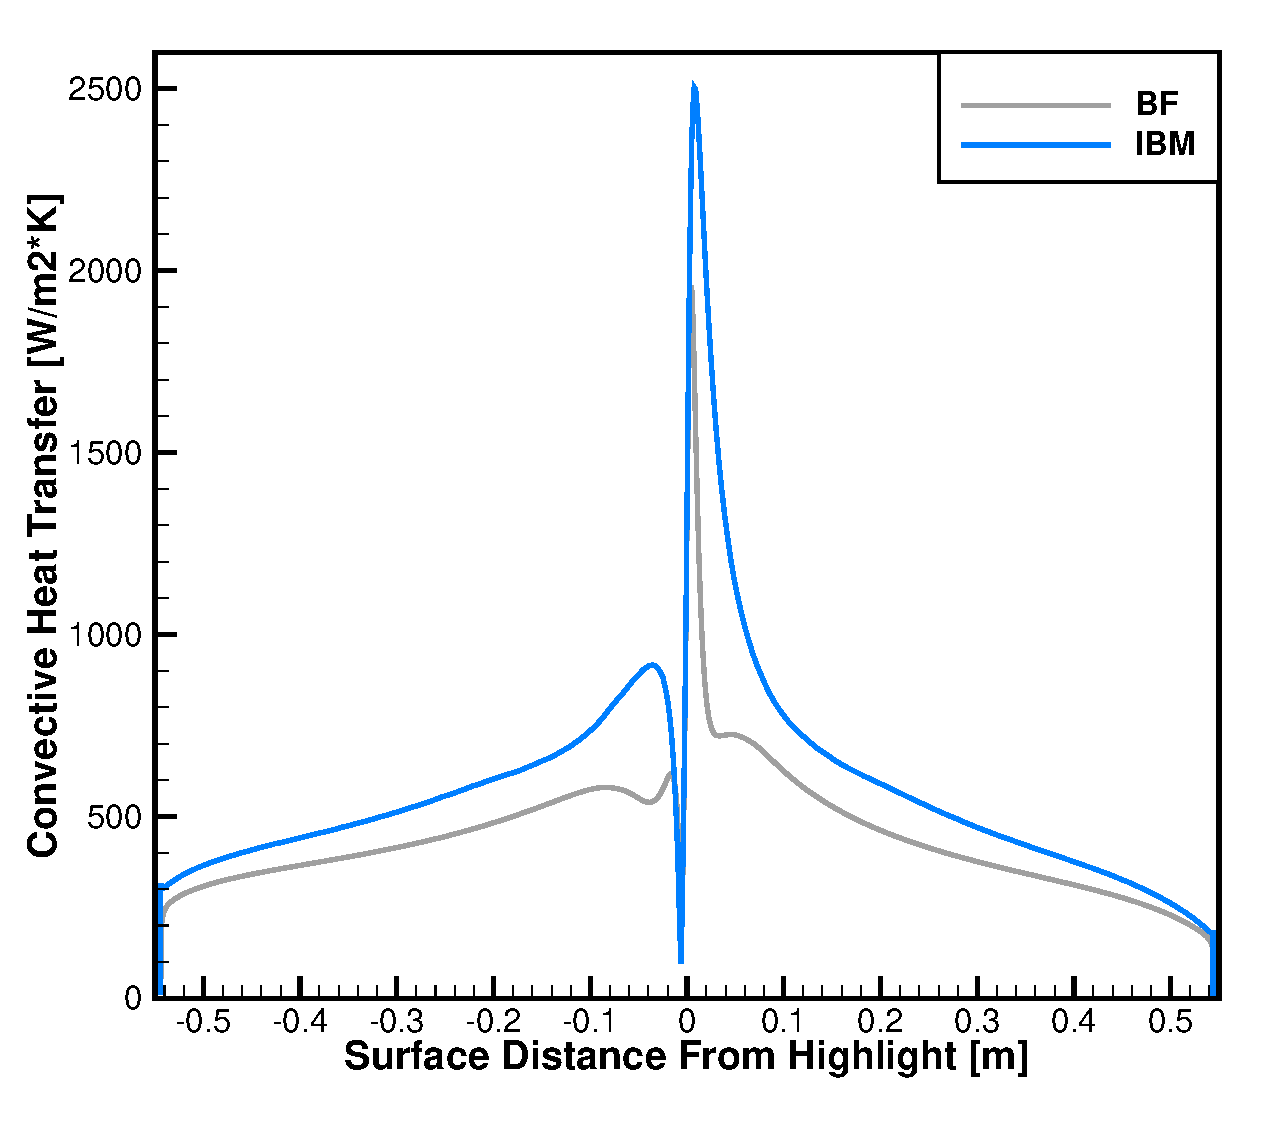
\includegraphics[trim={.1cm .1cm .1cm .1cm},clip,width=0.49\textwidth]{FIGURES/IBM_ARTICLE/CASE_04_HTC.eps}
    \label{ibm:fig:Case04HTC}%
    }
    \caption{Predicted ice shapes and convective heat transfer coefficient distributions for Case~04 using body-fitted and immersed-boundary formulations. The clean and experimental profiles are shown for reference in the ice-shape comparisons, together with predictions obtained using 1 and 5 accretion layers.}
    \label{ibm:fig:case04IceShapeHTC}
\end{figure}

These differences have a limited impact on the single-layer prediction, for which the body-fitted and immersed-boundary ice shapes remain close. In the multilayer simulation, however, small heat-transfer differences accumulate as the geometry is updated, leading to more visible deviations in the final ice shape. This effect is most noticeable near the lower horn, where the immersed-boundary solution predicts larger accretion.

Despite these differences, both approaches remain in good agreement with the experimental measurements and correctly reproduce the main glaze ice morphology, including the upper and lower horns. These results demonstrate the potential of the immersed-boundary framework for glaze ice accretion simulations, although the observed differences in local heat-transfer predictions indicate that this aspect requires further investigation.

\subsection{Case RG15}
\label{ibm:sec:rg15}

As a final demonstration, the immersed-boundary icing framework is applied to a 3D geometry based on the RG15 configuration considered during IPW2. The objective of this case is not to reproduce or validate the original workshop condition, but rather to provide a 3D test of the complete numerical framework.

The freestream conditions are defined by a Mach number of $M_\infty=0.07$, a Reynolds number of $Re=200$, a static temperature of $T_\infty=263.15$~K, and an angle of attack of $\alpha=4^\circ$. The reference chord is $C_{\mathrm{ref}}=0.3$~m. A liquid-water content of $\mathrm{LWC}=0.52$~g/m$^3$ is prescribed. An icing time of $20$~min is considered. Laminar-flow conditions are deliberately prescribed to alleviate the mesh-resolution requirements and associated element count. \addText{Consequently, no wall functions are employed, and the first layer of solid cells adjacent to the immersed surface is used for the ghost-cell treatment.}

Figure~\ref{ibm:fig:rg15Drop} first compares the collection-efficiency distributions obtained with the Eulerian and Lagrangian immersed-boundary formulations. The two approaches show good agreement in the predicted 3D impingement distributions along the leading edge, consistent with the agreement previously observed between the two droplet formulations using both body-fitted and immersed-boundary approaches.

\begin{figure}[htbp]
\centering
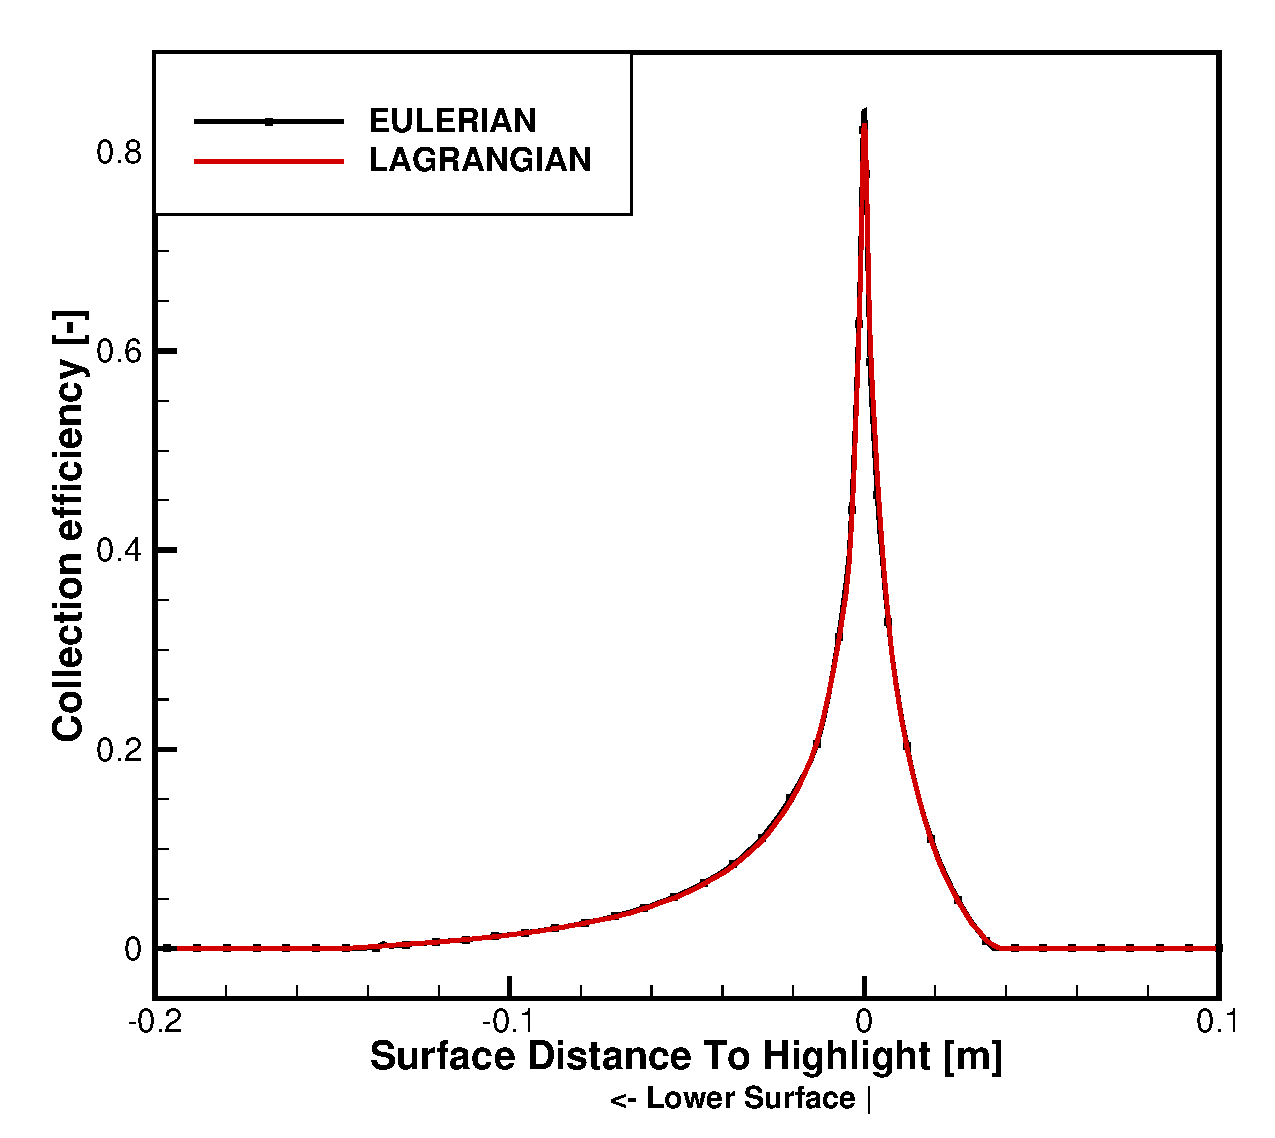
\includegraphics[width=0.6\textwidth]{FIGURES/IBM_ARTICLE/RG15_DROP_COMP.eps}
\caption{Comparison of the collection-efficiency distributions predicted by the Eulerian and Lagrangian immersed-boundary formulations for the RG15 configuration.}
\label{ibm:fig:rg15Drop}
\end{figure}

Figure~\ref{ibm:fig:rg15IceLayers} illustrates the evolution of the ice geometry through the successive accretion layers, while Figure~\ref{ibm:fig:rg15CleanIce} shows the clean wing together with the predicted ice geometry. The calculation demonstrates that the coupling between the immersed-boundary flow and droplet solvers and the level-set geometry-evolution methodology can be carried out for a 3D configuration. Following each geometry update, the extracted ice surface is introduced as the new immersed geometry while the aerodynamic and droplet calculations retain the non-conformal background mesh, thereby avoiding the generation of a new body-fitted RANS mesh.

\begin{figure}[htbp]
\centering
\subfloat[Evolution of the ice geometry through successive accretion layers.]{%
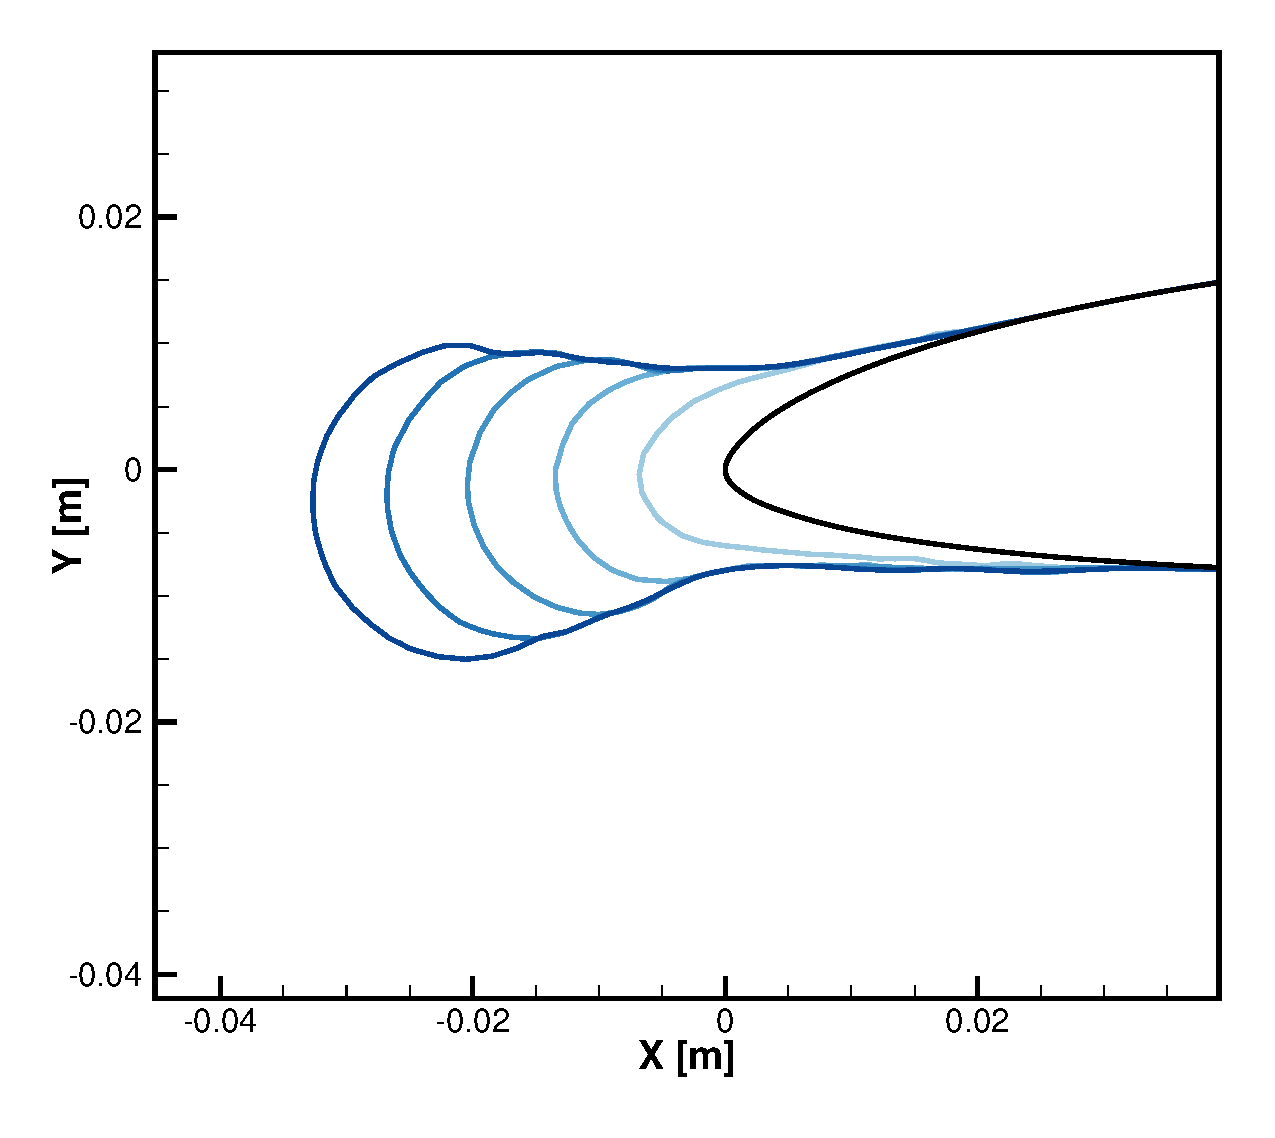
\includegraphics[width=0.48\textwidth]
{FIGURES/IBM_ARTICLE/RG15_IBM_3D.eps}
\label{ibm:fig:rg15IceLayers}%
}
\hfill
\subfloat[Clean wing and predicted ice shape.]{%
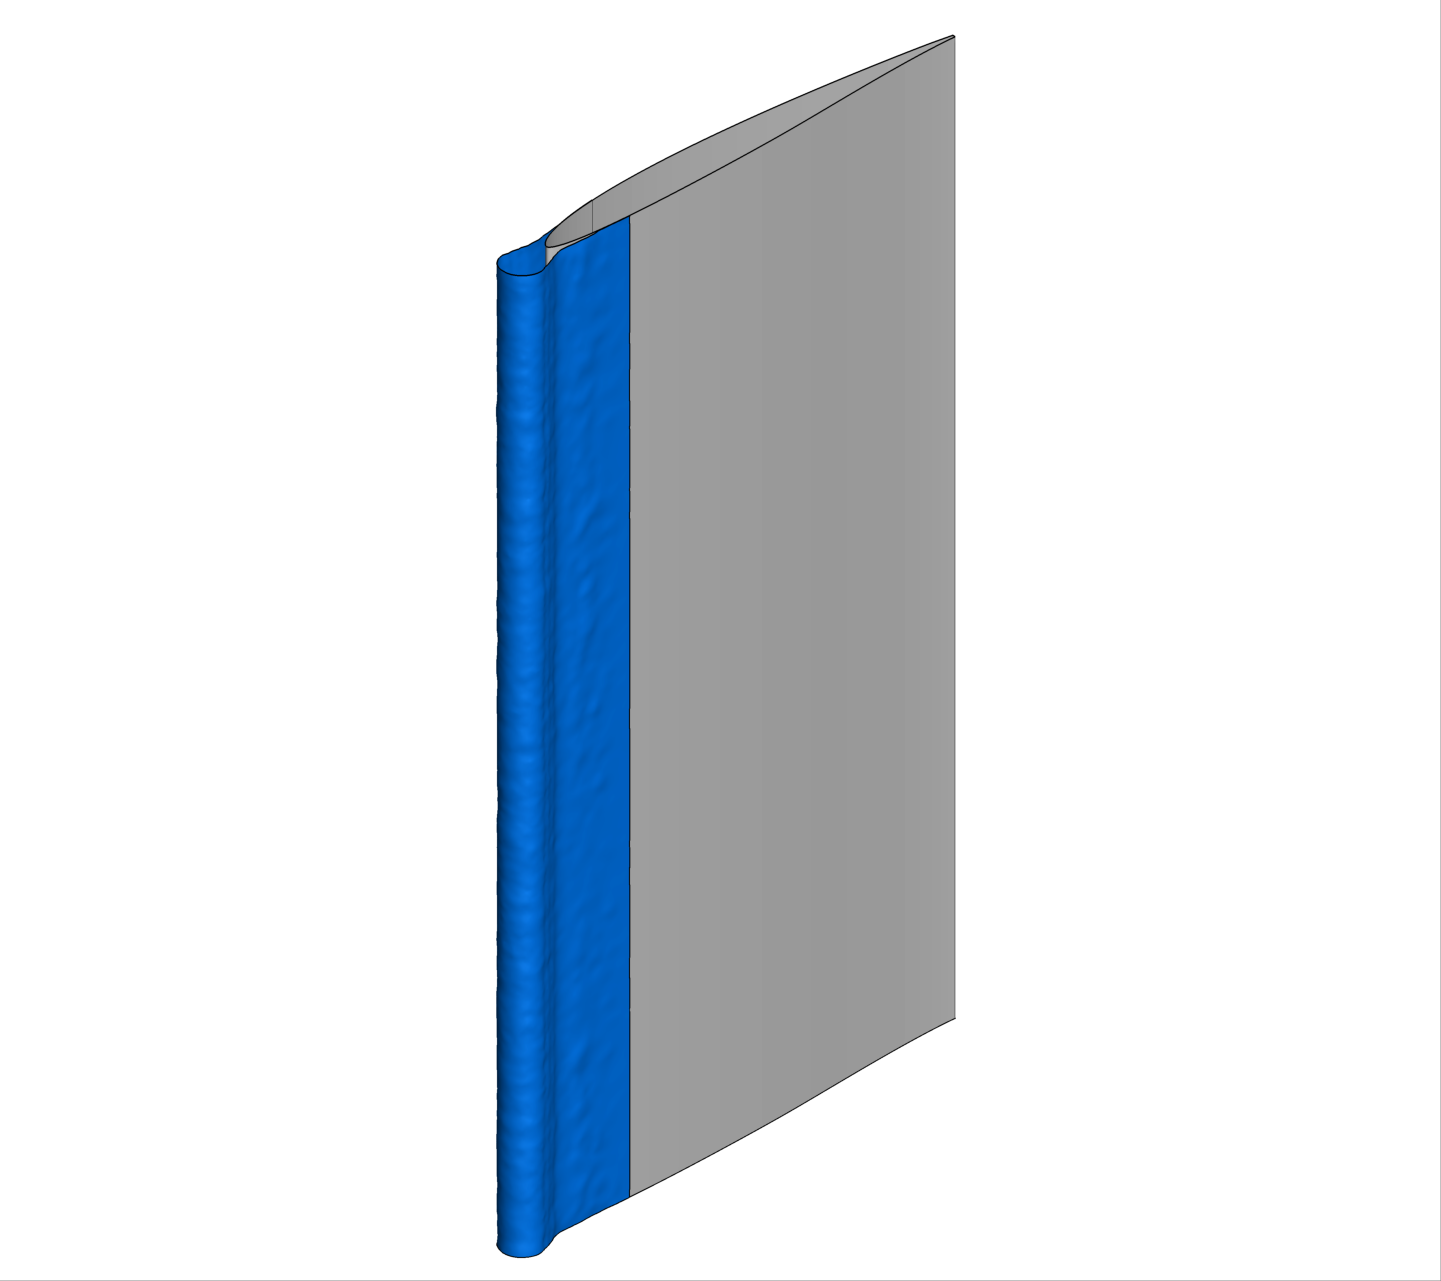
\includegraphics[width=0.48\textwidth]
{FIGURES/IBM_ARTICLE/RG15_3D_clean_and_ice.png}
\label{ibm:fig:rg15CleanIce}%
}
\caption{Predicted 3D ice accretion on the RG15 wing: (a) evolution of the ice geometry through successive accretion layers and (b) clean wing and predicted ice geometry.}
\label{ibm:fig:rg15Ice}
\end{figure}

At this stage, the case is intended as a demonstration of the 3D capability rather than a quantitative validation. The simplified laminar-flow assumption deliberately reduce the physical complexity of the original RG15 configuration and allow the numerical behavior of the coupled methodology to be examined independently of the additional complexities associated with turbulent wall modeling and glaze-ice thermodynamics.

\section{Conclusion}
\label{ibm:sec:conclusions}

This chapter extended the capabilities of an existing ghost-cell-based RANS immersed-boundary flow solver to ice accretion simulations. Eulerian and Lagrangian droplet transport formulations were adapted to the immersed geometry and integrated with the thermodynamic and geometry-evolution methodologies previously presented, resulting in a coupled immersed-boundary icing framework. The objective is to reduce the dependency on body-fitted mesh generation and deformation while preserving the accuracy required for aircraft icing simulations.

The framework was first verified using a canonical cylinder case with an analytical collection-efficiency solution. Both Eulerian and Lagrangian droplet solvers reproduced the theoretical distribution on body-fitted and immersed-boundary meshes.

The methodology was then assessed under SLD conditions using the \cite{papadakism2004water} benchmark. Including droplet splashing improved the agreement with experimental collection-efficiency data, with similar behavior observed for the body-fitted and immersed-boundary formulations.

Complete ice accretion simulations were then performed for rime and glaze conditions on a NACA~0012 airfoil from wind-tunnel experiments \cite{trontin2017description}. For the rime case, the body-fitted and immersed-boundary results were nearly identical and agreed well with the experimental profile. For the glaze case, both approaches reproduced the main ice-shape features, including horn formation, although differences in heat transfer led to deviations in the multilayer ice shapes.

Finally, the framework was applied to the 3D RG15 configuration under simplified laminar-flow condition. Consistent Eulerian and Lagrangian impingement distributions were obtained, and the multilayer simulation demonstrated the coupling of the immersed-boundary flow and droplet solvers with the level-set geometry-evolution methodology for a 3D configuration.

Future work will focus on improving the immersed-boundary aerodynamic and thermal wall treatments and assessing the methodology under more representative 3D aerodynamic and icing conditions.

\newpage
